\RequirePackage[l2tabu,orthodox]{nag} % Раскомментировав, можно в логе получать рекомендации относительно правильного использования пакетов и предупреждения об устаревших и нерекомендуемых пакетах
% Формат А4, 14pt (ГОСТ Р 7.0.11-2011, 5.3.6)
\documentclass[a4paper,14pt]{extreport}

%%% Проверка используемого TeX-движка %%%
\usepackage{iftex}[2013/04/04]
\newif\ifxetexorluatex   % определяем новый условный оператор (http://tex.stackexchange.com/a/47579/79756)
\ifXeTeX
    \xetexorluatextrue
\else
    \ifLuaTeX
        \xetexorluatextrue
    \else
        \xetexorluatexfalse
    \fi
\fi

%%% Поля и разметка страницы %%%
\usepackage{pdflscape}                              % Для включения альбомных страниц
\usepackage{geometry}                               % Для последующего задания полей

%%% Математические пакеты %%%
\usepackage{amsthm,amsfonts,amsmath,amssymb,amscd}  % Математические дополнения от AMS
\usepackage{mathtools}                              % Добавляет окружение multlined

%%%% Установки для размера шрифта 14 pt %%%%
%% Формирование переменных и констант для сравнения (один раз для всех подключаемых файлов)%%
%% должно располагаться до вызова пакета fontspec или polyglossia, потому что они сбивают его работу
\newlength{\curtextsize}
\newlength{\bigtextsize}
\setlength{\bigtextsize}{13.9pt}

\makeatletter
%\show\f@size                                       % неплохо для отслеживания, но вызывает стопорение процесса, если документ компилируется без команды  -interaction=nonstopmode 
\setlength{\curtextsize}{\f@size pt}
\makeatother

%%% Кодировки и шрифты %%%
\ifxetexorluatex
    \usepackage{polyglossia}[2014/05/21]            % Поддержка многоязычности (fontspec подгружается автоматически)
\else
    \RequirePDFTeX                                  % tests for PDFTEX use and throws an error if a different engine is being used
   %%% Решение проблемы копирования текста в буфер кракозябрами
%    \input glyphtounicode.tex
%    \input glyphtounicode-cmr.tex %from pdfx package
%    \pdfgentounicode=1
    \usepackage{cmap}                               % Улучшенный поиск русских слов в полученном pdf-файле
    \defaulthyphenchar=127                          % Если стоит до fontenc, то переносы не впишутся в выделяемый текст при копировании его в буфер обмена
    \usepackage[T2A]{fontenc}                       % Поддержка русских букв
    \usepackage[utf8]{inputenc}[2014/04/30]         % Кодировка utf8
    \usepackage[english, russian]{babel}[2014/03/24]% Языки: русский, английский
    \IfFileExists{pscyr.sty}{\usepackage{pscyr}}{}  % Красивые русские шрифты
\fi

%%% Оформление абзацев %%%
\usepackage{indentfirst}                            % Красная строка

%%% Цвета %%%
\usepackage[dvipsnames,usenames]{color}
\usepackage{colortbl}
%\usepackage[dvipsnames, table, hyperref, cmyk]{xcolor} % Вероятно, более новый вариант, вместо предыдущих двух строк. Конвертация всех цветов в cmyk заложена как удовлетворение возможного требования типографий. Возможно конвертирование и в rgb.

%%% Таблицы %%%
\usepackage{longtable}                              % Длинные таблицы
\usepackage{multirow,makecell,array}                % Улучшенное форматирование таблиц
\usepackage{booktabs}                               % Возможность оформления таблиц в классическом книжном стиле (при правильном использовании не противоречит ГОСТ)

%%% Общее форматирование
\usepackage{soulutf8}                               % Поддержка переносоустойчивых подчёркиваний и зачёркиваний
\usepackage{icomma}                                 % Запятая в десятичных дробях


%%% Гиперссылки %%%
\usepackage{hyperref}[2012/11/06]

%%% Изображения %%%
\usepackage{graphicx}[2014/04/25]                   % Подключаем пакет работы с графикой

%%% Списки %%%
\usepackage{enumitem}

%%% Подписи %%%
\usepackage{caption}[2013/05/02]                    % Для управления подписями (рисунков и таблиц) % Может управлять номерами рисунков и таблиц с caption %Иногда может управлять заголовками в списках рисунков и таблиц
\usepackage{subcaption}[2013/02/03]                 % Работа с подрисунками и подобным

%%% Интервалы %%%
\usepackage[onehalfspacing]{setspace}               % Опция запуска пакета правит не только интервалы в обычном тексте, но и формульные

%%% Счётчики %%%
\usepackage[figure,table]{totalcount}               % Счётчик рисунков и таблиц
\usepackage{totcount}                               % Пакет создания счётчиков на основе последнего номера подсчитываемого элемента (может требовать дважды компилировать документ)
\usepackage{totpages}                               % Счётчик страниц, совместимый с hyperref (ссылается на номер последней страницы). Желательно ставить последним пакетом в преамбуле

%%% Продвинутое управление групповыми ссылками (пока только формулами) %%%
\ifxetexorluatex
    \usepackage{cleveref}                           % cleveref корректно считывает язык из настроек polyglossia
\else
    \usepackage[russian]{cleveref}                  % cleveref имеет сложности со считыванием языка из babel. Такое решение русификации вывода выбрано вместо определения в documentclass из опасности что-то лишнее передать во все остальные пакеты, включая библиографию.
\fi
\creflabelformat{equation}{#2#1#3}                  % Формат по умолчанию ставил круглые скобки вокруг каждого номера ссылки, теперь просто номера ссылок без какого-либо дополнительного оформления

  % Пакеты общие для диссертации и автореферата
%%% Колонтитулы %%%
\usepackage{fancyhdr}

%%% Прикладные пакеты %%% 
\usepackage{calc}               % Пакет для расчётов параметров, например длины
%\usepackage{etoolbox}          % ради функции patchcmd для управления списком литературы

\usepackage {interfaces-base}   % Набор базовых интерфейсов к некоторым пакетам, конкретные реализации загружаются в стиле

%%% Заголовки %%%
\usepackage{titlesec}           % Пакет настройки шрифтов заголовков в тексте

%%% Оглавление %%%
\usepackage{tocloft}

%%% Счётчики %%%
\usepackage{chngcntr}           % оперативная перенастройка счётчиков         % Пакеты для диссертации
\usepackage{tabularx, tabu, tabulary}  %таблицы с автоматически подбирающейся шириной столбцов

% Листинги с исходным кодом программ
\usepackage{fancyvrb}
\usepackage{listings}

% Плавающие окружения. во многом лучше пакета float
\usepackage{floatrow}

% Русская традиция начертания греческих букв
%\usepackage{upgreek} % прямые греческие ради русской традиции        % Пакеты для специфических пользовательских задач

%%%%%%%%%%%%%%%%%%%%%%%%%%%%%%%%%%%%%%%%%%%%%%%%%%%%%%
%%%% Файл упрощённых настроек шаблона диссертации %%%%
%%%%%%%%%%%%%%%%%%%%%%%%%%%%%%%%%%%%%%%%%%%%%%%%%%%%%%

%%%        Подключение пакетов                 %%%
\usepackage{ifthen}                 % добавляет ifthenelse
%%% Инициализирование переменных, не трогать!  %%%
\newcounter{intvl}
\newcounter{otstup}
\newcounter{contnumeq}
\newcounter{contnumfig}
\newcounter{contnumtab}
\newcounter{pgnum}
\newcounter{bibliosel}
\newcounter{chapstyle}
\newcounter{headingdelim}
\newcounter{headingalign}
\newcounter{headingsize}
\newcounter{tabcap}
\newcounter{tablaba}
\newcounter{tabtita}
%%%%%%%%%%%%%%%%%%%%%%%%%%%%%%%%%%%%%%%%%%%%%%%%%%

%%% Область упрощённого управления оформлением %%%

%% Интервал между заголовками и между заголовком и текстом
% Заголовки отделяют от текста сверху и снизу тремя интервалами (ГОСТ Р 7.0.11-2011, 5.3.5)
\setcounter{intvl}{3}               % Коэффициент кратности к размеру шрифта

%% Отступы у заголовков в тексте
\setcounter{otstup}{0}              % 0 --- без отступа; 1 --- абзацный отступ

%% Нумерация формул, таблиц и рисунков
\setcounter{contnumeq}{0}           % Нумерация формул: 0 --- пораздельно (во введении подряд, без номера раздела); 1 --- сквозная нумерация по всей диссертации
\setcounter{contnumfig}{0}          % Нумерация рисунков: 0 --- пораздельно (во введении подряд, без номера раздела); 1 --- сквозная нумерация по всей диссертации
\setcounter{contnumtab}{1}          % Нумерация таблиц: 0 --- пораздельно (во введении подряд, без номера раздела); 1 --- сквозная нумерация по всей диссертации

%% Оглавление
\setcounter{pgnum}{1}               % 0 --- номера страниц никак не обозначены; 1 --- Стр. над номерами страниц (дважды компилировать после изменения)

%% Библиография
\setcounter{bibliosel}{1}           % 0 --- встроенная реализация с загрузкой файла через движок bibtex8; 1 --- реализация пакетом biblatex через движок biber

%% Текст и форматирование заголовков
\setcounter{chapstyle}{0}           % 0 --- разделы только под номером; 1 --- разделы с названием "Глава" перед номером
\setcounter{headingdelim}{1}        % 0 --- номер отделен пропуском в 1em или \quad; 1 --- номера разделов и приложений отделены точкой с пробелом, подразделы пропуском без точки; 2 --- номера разделов, подразделов и приложений отделены точкой с пробелом.

%% Выравнивание заголовков в тексте
\setcounter{headingalign}{0}        % 0 --- по центру; 1 --- по левому краю

%% Размеры заголовков в тексте
\setcounter{headingsize}{0}         % 0 --- по ГОСТ, все всегда 14 пт; 1 --- пропорционально изменяющийся размер в зависимости от базового шрифта

%% Подпись таблиц
\setcounter{tabcap}{0}              % 0 --- по ГОСТ, номер таблицы и название разделены тире, выровнены по левому краю, при необходимости на нескольких строках; 1 --- подпись таблицы не по ГОСТ, на двух и более строках, дальнейшие настройки: 
%Выравнивание первой строки, с подписью и номером
\setcounter{tablaba}{2}             % 0 --- по левому краю; 1 --- по центру; 2 --- по правому краю
%Выравнивание строк с самим названием таблицы
\setcounter{tabtita}{1}             % 0 --- по левому краю; 1 --- по центру; 2 --- по правому краю

%%% Цвета гиперссылок %%%
% Latex color definitions: http://latexcolor.com/
\definecolor{linkcolor}{rgb}{0.9,0,0}
\definecolor{citecolor}{rgb}{0,0.6,0}
\definecolor{urlcolor}{rgb}{0,0,1}
%\definecolor{linkcolor}{rgb}{0,0,0} %black
%\definecolor{citecolor}{rgb}{0,0,0} %black
%\definecolor{urlcolor}{rgb}{0,0,0} %black                    % Упрощённые настройки шаблона

%%% Переопределение именований, чтобы можно было и в преамбуле использовать %%%
\renewcommand{\chaptername}{Глава}
\renewcommand{\appendixname}{Приложение} % (ГОСТ Р 7.0.11-2011, 5.7)
       % Переопределение именований, чтобы можно было и в преамбуле использовать
% Новые переменные, которые могут использоваться во всём проекте
% ГОСТ 7.0.11-2011
% 9.2 Оформление текста автореферата диссертации
% 9.2.1 Общая характеристика работы включает в себя следующие основные структурные
% элементы:
% актуальность темы исследования;
\newcommand{\actualityTXT}{Актуальность темы.}
% степень ее разработанности;
\newcommand{\progressTXT}{Степень разработанности темы.}
% цели и задачи;
\newcommand{\aimTXT}{Цель работы:}
\newcommand{\tasksTXT}{задачи}
% научную новизну;
\newcommand{\noveltyTXT}{Научная новизна:}
% теоретическую и практическую значимость работы;
%\newcommand{\influenceTXT}{Теоретическая и практическая значимость}
% или чаще используют просто
\newcommand{\influenceTXT}{Практическая значимость}
% методологию и методы исследования;
\newcommand{\methodsTXT}{Mетодология и методы исследования.}
% положения, выносимые на защиту;
\newcommand{\defpositionsTXT}{Основные положения, выносимые на~защиту:}
% степень достоверности и апробацию результатов.
\newcommand{\reliabilityTXT}{Достоверность}
\newcommand{\probationTXT}{Апробация работы.}

\newcommand{\contributionTXT}{Личный вклад.}
\newcommand{\publicationsTXT}{Публикации.}


\newcommand{\authorbibtitle}{Публикации автора по теме диссертации}
\newcommand{\fullbibtitle}{Список литературы} % (ГОСТ Р 7.0.11-2011, 4)
  % Новые переменные, которые могут использоваться во всём проекте

%%% Основные сведения %%%
\newcommand{\thesisAuthor}             % Диссертация, ФИО автора
{%
    \texorpdfstring{% \texorpdfstring takes two arguments and uses the first for (La)TeX and the second for pdf
        Ефанов Андрей Александрович% так будет отображаться на титульном листе или в тексте, где будет использоваться переменная
    }{%
        Ефанов Андрей Александрович% эта запись для свойств pdf-файла. В таком виде, если pdf будет обработан программами для сбора библиографических сведений, будет правильно представлена фамилия.
    }%
}
\newcommand{\thesisAuthorShort}             % Диссертация, ФИО автора инициалами
{А.А.~Ефанов}

\newcommand{\kafedra}                % Кафедра
{Кафедра Прикладной Математики}
\newcommand{\thesisTitle}              % Диссертация, название
{\texorpdfstring{Разработка экспертной ситсемы в среде CLIPS}{Разработка экспертной ситсемы в среде CLIPS}}
\newcommand{\courseName}
{Экспертные системы}
\newcommand{\labNumber}
{2}
\newcommand{\thesisCity}               % Диссертация, город защиты
{Москва}
\newcommand{\thesisYear}               % Диссертация, год защиты
{2017}
\newcommand{\thesisOrganization}       % Диссертация, организация
{Национальный исследовательский университет}

\newcommand{\supervisorFio}            % Научный руководитель, ФИО
{Еремеев Александр Павлович}
\newcommand{\supervisorFioShort}            % Научный руководитель, ФИО
{А.П.~Еремеев}


% To avoid conflict with beamer class use \providecommand
\providecommand{\keywords}%                 % Ключевые слова для метаданных PDF диссертации и автореферата
{}      % Основные сведения
%%% Макет страницы %%%
% Выставляем значения полей (ГОСТ 7.0.11-2011, 5.3.7)
\geometry{a4paper,top=2cm,bottom=2cm,left=2.5cm,right=1cm}

%%% Кодировки и шрифты %%%
\ifxetexorluatex
    \setmainlanguage[babelshorthands=true]{russian}  % Язык по-умолчанию русский с поддержкой приятных команд пакета babel
    \setotherlanguage{english}                       % Дополнительный язык = английский (в американской вариации по-умолчанию)
    \setmonofont{Courier New}
    \newfontfamily\cyrillicfonttt{Courier New}
    \ifXeTeX
        \defaultfontfeatures{Ligatures=TeX,Mapping=tex-text}
    \else
        \defaultfontfeatures{Ligatures=TeX}
    \fi
    \setmainfont{Times New Roman}
    \newfontfamily\cyrillicfont{Times New Roman}
    \setsansfont{Arial}
    \newfontfamily\cyrillicfontsf{Arial}
\else
    \IfFileExists{pscyr.sty}{\renewcommand{\rmdefault}{ftm}}{}
\fi

%%% Интервалы %%%
%linespread-реализация ближе к реализации полуторного интервала в ворде.
%setspace реализация заточена под шрифты 10, 11, 12pt, под остальные кегли хуже, но всё же ближе к типографской классике. 
%\linespread{1.42}                    % Полуторный интервал (ГОСТ Р 7.0.11-2011, 5.3.6)

%%% Выравнивание и переносы %%%
\sloppy                             % Избавляемся от переполнений
\clubpenalty=10000                  % Запрещаем разрыв страницы после первой строки абзаца
\widowpenalty=10000                 % Запрещаем разрыв страницы после последней строки абзаца

%%% Подписи %%%
\captionsetup{%
singlelinecheck=off,                % Многострочные подписи, например у таблиц
skip=2pt,                           % Вертикальная отбивка между подписью и содержимым рисунка или таблицы определяется ключом
justification=centering,            % Центрирование подписей, заданных командой \caption
}

%%% Рисунки %%%
\DeclareCaptionLabelSeparator*{emdash}{~--- }             % (ГОСТ 2.105, 4.3.1)
\captionsetup[figure]{labelsep=emdash,font=onehalfspacing,position=bottom}

%%% Таблицы %%%
\ifthenelse{\equal{\thetabcap}{0}}{%
    \newcommand{\tabcapalign}{\raggedright}  % по левому краю страницы или аналога parbox
}

\ifthenelse{\equal{\thetablaba}{0} \AND \equal{\thetabcap}{1}}{%
    \newcommand{\tabcapalign}{\raggedright}  % по левому краю страницы или аналога parbox
}

\ifthenelse{\equal{\thetablaba}{1} \AND \equal{\thetabcap}{1}}{%
    \newcommand{\tabcapalign}{\centering}    % по центру страницы или аналога parbox
}

\ifthenelse{\equal{\thetablaba}{2} \AND \equal{\thetabcap}{1}}{%
    \newcommand{\tabcapalign}{\raggedleft}   % по правому краю страницы или аналога parbox
}

\ifthenelse{\equal{\thetabtita}{0} \AND \equal{\thetabcap}{1}}{%
    \newcommand{\tabtitalign}{\raggedright}  % по левому краю страницы или аналога parbox
}

\ifthenelse{\equal{\thetabtita}{1} \AND \equal{\thetabcap}{1}}{%
    \newcommand{\tabtitalign}{\centering}    % по центру страницы или аналога parbox
}

\ifthenelse{\equal{\thetabtita}{2} \AND \equal{\thetabcap}{1}}{%
    \newcommand{\tabtitalign}{\raggedleft}   % по правому краю страницы или аналога parbox
}

\DeclareCaptionFormat{tablenocaption}{\tabcapalign #1\strut}        % Наименование таблицы отсутствует
\ifthenelse{\equal{\thetabcap}{0}}{%
    \DeclareCaptionFormat{tablecaption}{\tabcapalign #1#2#3}
    \captionsetup[table]{labelsep=emdash}                       % тире как разделитель идентификатора с номером от наименования
}{%
    \DeclareCaptionFormat{tablecaption}{\tabcapalign #1#2\par%  % Идентификатор таблицы на отдельной строке
        \tabtitalign{#3}}                                       % Наименование таблицы строкой ниже
    \captionsetup[table]{labelsep=space}                        % пробельный разделитель идентификатора с номером от наименования
}
\captionsetup[table]{format=tablecaption,singlelinecheck=off,font=onehalfspacing,position=top,skip=0pt}  % многострочные наименования и прочее
\DeclareCaptionLabelFormat{continued}{Продолжение таблицы~#2}

%%% Подписи подрисунков %%%
\renewcommand{\thesubfigure}{\asbuk{subfigure}}           % Буквенные номера подрисунков
\captionsetup[subfigure]{font={normalsize},               % Шрифт подписи названий подрисунков (не отличается от основного)
    labelformat=brace,                                    % Формат обозначения подрисунка
    justification=centering,                              % Выключка подписей (форматирование), один из вариантов            
}
%\DeclareCaptionFont{font12pt}{\fontsize{12pt}{13pt}\selectfont} % объявляем шрифт 12pt для использования в подписях, тут же надо интерлиньяж объявлять, если не наследуется
%\captionsetup[subfigure]{font={font12pt}}                 % Шрифт подписи названий подрисунков (всегда 12pt)

%%% Настройки гиперссылок %%%
\ifLuaTeX
    \hypersetup{
        unicode,                % Unicode encoded PDF strings
    }
\fi

\hypersetup{
    linktocpage=true,           % ссылки с номера страницы в оглавлении, списке таблиц и списке рисунков
%    linktoc=all,                % both the section and page part are links
%    pdfpagelabels=false,        % set PDF page labels (true|false)
    plainpages=false,           % Forces page anchors to be named by the Arabic form  of the page number, rather than the formatted form
    colorlinks,                 % ссылки отображаются раскрашенным текстом, а не раскрашенным прямоугольником, вокруг текста
    linkcolor={linkcolor},      % цвет ссылок типа ref, eqref и подобных
    citecolor={citecolor},      % цвет ссылок-цитат
    urlcolor={urlcolor},        % цвет гиперссылок
%    hidelinks,                  % Hide links (removing color and border)
    pdftitle={\courseName},    % Заголовок
    pdfauthor={\thesisAuthor},  % Автор
    pdfsubject={}%\thesisSpecialtyNumber\ \thesisSpecialtyTitle},      % Тема
%    pdfcreator={Создатель},     % Создатель, Приложение
%    pdfproducer={Производитель},% Производитель, Производитель PDF
    pdfkeywords={\keywords},    % Ключевые слова
    pdflang={ru},
}

%%% Шаблон %%%
\DeclareRobustCommand{\todo}{\textcolor{red}}       % решаем проблему превращения названия цвета в результате \MakeUppercase, http://tex.stackexchange.com/a/187930/79756 , \DeclareRobustCommand protects \todo from expanding inside \MakeUppercase
\setlength{\parindent}{2.5em}                       % Абзацный отступ. Должен быть одинаковым по всему тексту и равен пяти знакам (ГОСТ Р 7.0.11-2011, 5.3.7).

%%% Списки %%%
% Используем короткое тире (endash) для ненумерованных списков (ГОСТ 2.105-95, пункт 4.1.7, требует дефиса, но так лучше смотрится)
\renewcommand{\labelitemi}{\normalfont\bfseries{--}}

% Перечисление строчными буквами латинского алфавита (ГОСТ 2.105-95, 4.1.7)
%\renewcommand{\theenumi}{\alph{enumi}}
%\renewcommand{\labelenumi}{\theenumi)} 

% Перечисление строчными буквами русского алфавита (ГОСТ 2.105-95, 4.1.7)
%\makeatletter
%\AddEnumerateCounter{\asbuk}{\russian@alph}{щ}      % Управляем списками/перечислениями через пакет enumitem, а он 'не знает' про asbuk, потому 'учим' его
%\makeatother
%\renewcommand{\theenumi}{\asbuk{enumi}}
%\renewcommand{\labelenumi}{\theenumi)} 

\setlist{nosep,%                                    % Единый стиль для всех списков (пакет enumitem), без дополнительных интервалов.
    labelindent=\parindent,leftmargin=*%            % Каждый пункт, подпункт и перечисление записывают с абзацного отступа (ГОСТ 2.105-95, 4.1.8)
}
    % Стили общие для диссертации и автореферата
%%% Изображения %%%
\graphicspath{{images/}{Dissertation/images/}}         % Пути к изображениям

\LoadInterface {titlesec}                   % Подгружаем интерфейсы для дополнительных опций управления некоторыми пакетами

%%% Блок управления параметрами для выравнивания заголовков в тексте %%%
\newlength{\otstuplen}
\setlength{\otstuplen}{\theotstup\parindent}
\ifthenelse{\equal{\theheadingalign}{0}}{% выравнивание заголовков в тексте
    \newcommand{\hdngalign}{\filcenter}                % по центру
    \newcommand{\hdngaligni}{\hfill\hspace{\otstuplen}}% по центру
}{%
    \newcommand{\hdngalign}{\filright}                 % по левому краю
    \newcommand{\hdngaligni}{\hspace{\otstuplen}}      % по левому краю
} % В обоих случаях вроде бы без переноса, как и надо (ГОСТ Р 7.0.11-2011, 5.3.5)

%%% Оглавление %%%
\renewcommand{\cftchapdotsep}{\cftdotsep}                % отбивка точками до номера страницы начала главы/раздела
\renewcommand{\cfttoctitlefont}{\hdngaligni\fontsize{14pt}{16pt}\selectfont\bfseries}% вместе со следующей строкой
\renewcommand{\cftaftertoctitle}{\hfill}                 % устанавливает заголовок по центру
\setlength{\cftbeforetoctitleskip}{-1.4\curtextsize}     % Поскольку этот заголовок всегда является первым на странице, то перед ним отделять пустым тройным интервалом не следует. Независимо от основного шрифта, в этом случае зануление (почти) происходит при -1.4\curtextsize.
\setlength{\cftaftertoctitleskip}{\theintvl\curtextsize} % Если считаем Оглавление заголовком, то выставляем после него тройной интервал через наше определённое значение

%% Переносить слова в заголовке не допускается (ГОСТ Р 7.0.11-2011, 5.3.5). Заголовки в оглавлении должны точно повторять заголовки в тексте (ГОСТ Р 7.0.11-2011, 5.2.3). Прямого указания на запрет переносов в оглавлении нет, но по той же логике невнесения искажений в смысл, лучше в оглавлении не переносить:
\cftsetrmarg{2.55em plus1fil}                       %To have the (sectional) titles in the ToC, etc., typeset ragged right with no hyphenation
\renewcommand{\cftchappagefont}{\normalfont}        % нежирные номера страниц у глав в оглавлении
\renewcommand{\cftchapleader}{\cftdotfill{\cftchapdotsep}}% нежирные точки до номеров страниц у глав в оглавлении
%\renewcommand{\cftchapfont}{}                       % нежирные названия глав в оглавлении

\ifthenelse{\theheadingdelim > 0}{%
    \renewcommand\cftchapaftersnum{.\ }   % добавляет точку с пробелом после номера раздела в оглавлении
}{%
\renewcommand\cftchapaftersnum{\quad}     % добавляет \quad после номера раздела в оглавлении
}
\ifthenelse{\theheadingdelim > 1}{%
    \renewcommand\cftsecaftersnum{.\ }    % добавляет точку с пробелом после номера подраздела в оглавлении
    \renewcommand\cftsubsecaftersnum{.\ } % добавляет точку с пробелом после номера подподраздела в оглавлении
}{%
\renewcommand\cftsecaftersnum{\quad}      % добавляет \quad после номера подраздела в оглавлении
\renewcommand\cftsubsecaftersnum{\quad}   % добавляет \quad после номера подподраздела в оглавлении
}

\ifthenelse{\equal{\thepgnum}{1}}{%
    \addtocontents{toc}{~\hfill{Стр.}\par}% добавить Стр. над номерами страниц
}

%%% Оформление названий глав %%%
%% настройки заголовка списка рисунков
\renewcommand{\cftloftitlefont}{\hdngaligni\fontsize{14pt}{16pt}\selectfont\bfseries}% вместе со следующей строкой
\renewcommand{\cftafterloftitle}{\hfill}                                             % устанавливает заголовок по центру
\setlength{\cftbeforeloftitleskip}{-1.5\curtextsize}     % Поскольку этот заголовок всегда является первым на странице, то перед ним отделять пустым тройным интервалом не следует. Независимо от основного шрифта, в этом случае зануление (почти) происходит при -1.5\curtextsize.
\setlength{\cftafterloftitleskip}{\theintvl\curtextsize} % выставляем после него тройной интервал через наше определённое значение

%% настройки заголовка списка таблиц
\renewcommand{\cftlottitlefont}{\hdngaligni\fontsize{14pt}{16pt}\selectfont\bfseries}% вместе со следующей строкой
\renewcommand{\cftafterlottitle}{\hfill}                                             % устанавливает заголовок по центру
\setlength{\cftbeforelottitleskip}{-1.5\curtextsize}     % Поскольку этот заголовок всегда является первым на странице, то перед ним отделять пустым тройным интервалом не следует. Независимо от основного шрифта, в этом случае зануление (почти) происходит при -1.5\curtextsize.
\setlength{\cftafterlottitleskip}{\theintvl\curtextsize} % выставляем после него тройной интервал через наше определённое значение

\ifnum\curtextsize>\bigtextsize     % Проверяем условие использования базового шрифта 14 pt
\setlength{\headheight}{17pt}       % Исправляем высоту заголовка
\else
\setlength{\headheight}{15pt}       % Исправляем высоту заголовка
\fi

%%% Колонтитулы %%%
% Порядковый номер страницы печатают на середине верхнего поля страницы (ГОСТ Р 7.0.11-2011, 5.3.8)
\makeatletter
\let\ps@plain\ps@fancy              % Подчиняем первые страницы каждой главы общим правилам
\makeatother
\pagestyle{fancy}                   % Меняем стиль оформления страниц
\fancyhf{}                          % Очищаем текущие значения
\fancyhead[C]{\thepage}             % Печатаем номер страницы на середине верхнего поля
\renewcommand{\headrulewidth}{0pt}  % Убираем разделительную линию

%%% Оформление заголовков глав, разделов, подразделов %%%
%% Работа должна быть выполнена ... размером шрифта 12-14 пунктов (ГОСТ Р 7.0.11-2011, 5.3.8). То есть не должно быть надписей шрифтом более 14. Так и поставим.
%% Эти установки будут давать одинаковый результат независимо от выбора базовым шрифтом 12 пт или 14 пт
\titleformat{\chapter}[block]                                % default display;  hang = with a hanging label. (Like the standard \section.); block = typesets the whole title in a block (a paragraph) without additional formatting. Useful in centered titles
        {\hdngalign\fontsize{14pt}{16pt}\selectfont\bfseries}% 
        %\fontsize{<size>}{<skip>} % второе число ставим 1.2*первое, чтобы адекватно отрабатывали команды по расчету полуторного интервала (домножая разные комбинации коэффициентов на этот)
        {\thechapter\cftchapaftersnum}                       % Заголовки в оглавлении должны точно повторять заголовки в тексте (ГОСТ Р 7.0.11-2011, 5.2.3).
        {0em}% отступ от номера до текста
        {}%

\titleformat{\section}[block]                                % default hang;  hang = with a hanging label. (Like the standard \section.); block = typesets the whole title in a block (a paragraph) without additional formatting. Useful in centered titles
        {\hdngalign\fontsize{14pt}{16pt}\selectfont\bfseries}% 
        %\fontsize{<size>}{<skip>} % второе число ставим 1.2*первое, чтобы адекватно отрабатывали команды по расчету полуторного интервала (домножая разные комбинации коэффициентов на этот)
        {\thesection\cftsecaftersnum}                        % Заголовки в оглавлении должны точно повторять заголовки в тексте (ГОСТ Р 7.0.11-2011, 5.2.3).
        {0em}% отступ от номера до текста
        {}%

\titleformat{\subsection}[block]                             % default hang;  hang = with a hanging label. (Like the standard \section.); block = typesets the whole title in a block (a paragraph) without additional formatting. Useful in centered titles
        {\hdngalign\fontsize{14pt}{16pt}\selectfont\bfseries}% 
        %\fontsize{<size>}{<skip>} % второе число ставим 1.2*первое, чтобы адекватно отрабатывали команды по расчету полуторного интервала (домножая разные комбинации коэффициентов на этот)
        {\thesubsection\cftsubsecaftersnum}                  % Заголовки в оглавлении должны точно повторять заголовки в тексте (ГОСТ Р 7.0.11-2011, 5.2.3).
        {0em}% отступ от номера до текста
        {}%

\ifthenelse{\equal{\thechapstyle}{1}}{%
    \sectionformat{\chapter}{% Параметры заголовков разделов в тексте
        label=\chaptername\ \thechapter\cftchapaftersnum,
        labelsep=0em,
    }
    %% Следующие две строки: будет вписано слово Глава перед каждым номером раздела в оглавлении   
    \renewcommand{\cftchappresnum}{\chaptername\ }
    \setlength{\cftchapnumwidth}{\widthof{\cftchapfont\cftchappresnum\thechapter\cftchapaftersnum}}
}%

%% Интервалы между заголовками
% На эти величины titlespacing множит через *
\beforetitleunit=\curtextsize% привязались к нашему размеру шрифта
\aftertitleunit=\curtextsize% привязались к нашему размеру шрифта

% Счётчик intvl и длина \otstup определены в файле setup
\titlespacing{\chapter}{\theotstup\parindent}{-1.7em}{*\theintvl}       % Заголовки отделяют от текста сверху и снизу тремя интервалами (ГОСТ Р 7.0.11-2011, 5.3.5). Поскольку название главы всегда является первым на странице, то перед ним отделять пустым тройным интервалом не следует. Независимо от основного шрифта, в этом случае зануление происходит при -1.7em.
\titlespacing{\section}{\theotstup\parindent}{*\theintvl}{*\theintvl}
\titlespacing{\subsection}{\theotstup\parindent}{*\theintvl}{*\theintvl}
\titlespacing{\subsubsection}{\theotstup\parindent}{*\theintvl}{*\theintvl}

%%% Блок дополнительного управления размерами заголовков
\ifthenelse{\equal{\theheadingsize}{1}}{% Пропорциональные заголовки и базовый шрифт 14 пт
    \renewcommand{\cfttoctitlefont}{\hdngaligni\Large\bfseries} % Исправляем размер заголовка оглавления
    \setlength{\cftbeforetoctitleskip}{-1.2\curtextsize}        % Исправляем вертикальный отступ перед заголовком оглавления
    \renewcommand{\cftloftitlefont}{\hdngaligni\Large\bfseries} % Исправляем размер заголовка списка рисунков
    \setlength{\cftbeforeloftitleskip}{-1.4\curtextsize}        % Исправляем вертикальный отступ перед заголовком списка рисунков
    \renewcommand{\cftlottitlefont}{\hdngaligni\Large\bfseries} % Исправляем размер заголовка списка таблиц 
    \setlength{\cftbeforelottitleskip}{-1.4\curtextsize}        % Исправляем вертикальный отступ перед заголовком списка таблиц
    \sectionformat{\chapter}{% Параметры заголовков разделов в тексте
        format=\hdngalign\Large\bfseries, % Исправляем размер заголовка
        top-=0.4em,                       % Исправляем вертикальный отступ перед заголовком
    }
    \sectionformat{\section}{% Параметры заголовков подразделов в тексте
        format=\hdngalign\large\bfseries, % Исправляем размер заголовка
    }
}

\ifthenelse{\equal{\theheadingsize}{1}\AND \curtextsize < \bigtextsize}{% Пропорциональные заголовки и базовый шрифт 14 пт
    \sectionformat{\chapter}{% Параметры заголовков разделов в тексте
        top-=0.2em, % Исправляем вертикальный отступ перед заголовком
    }
}

%%% Счётчики %%%

%% Упрощённые настройки шаблона диссертации: нумерация формул, таблиц, рисунков
\ifthenelse{\equal{\thecontnumeq}{1}}{%
    \counterwithout{equation}{chapter} % Убираем связанность номера формулы с номером главы/раздела
}
\ifthenelse{\equal{\thecontnumfig}{1}}{%
    \counterwithout{figure}{chapter}   % Убираем связанность номера рисунка с номером главы/раздела
}
\ifthenelse{\equal{\thecontnumtab}{1}}{%
    \counterwithout{table}{chapter}    % Убираем связанность номера таблицы с номером главы/раздела
}


%%http://www.linux.org.ru/forum/general/6993203#comment-6994589 (используется totcount)
\makeatletter
\def\formbytotal#1#2#3#4#5{%
    \newcount\@c
    \@c\totvalue{#1}\relax
    \newcount\@last
    \newcount\@pnul
    \@last\@c\relax
    \divide\@last 10
    \@pnul\@last\relax
    \divide\@pnul 10
    \multiply\@pnul-10
    \advance\@pnul\@last
    \multiply\@last-10
    \advance\@last\@c
    \total{#1}~#2%
    \ifnum\@pnul=1#5\else%
    \ifcase\@last#5\or#3\or#4\or#4\or#4\else#5\fi
    \fi
}
\makeatother

\AtBeginDocument{
%% регистрируем счётчики в системе totcounter
    \regtotcounter{totalcount@figure}
    \regtotcounter{totalcount@table}       % Если иным способом поставить в преамбуле то ошибка в числе таблиц
    \regtotcounter{TotPages}               % Если иным способом поставить в преамбуле то ошибка в числе страниц
}           % Стили для диссертации
% для вертикального центрирования ячеек в tabulary
\def\zz{\ifx\[$\else\aftergroup\zzz\fi}
\def\zzz{\setbox0\lastbox
\dimen0\dimexpr\extrarowheight + \ht0-\dp0\relax
\setbox0\hbox{\raise-.5\dimen0\box0}%
\ht0=\dimexpr\ht0+\extrarowheight\relax
\dp0=\dimexpr\dp0+\extrarowheight\relax 
\box0
}



\lstdefinelanguage{Renhanced}%
{keywords={abbreviate,abline,abs,acos,acosh,action,add1,add,%
        aggregate,alias,Alias,alist,all,anova,any,aov,aperm,append,apply,%
        approx,approxfun,apropos,Arg,args,array,arrows,as,asin,asinh,%
        atan,atan2,atanh,attach,attr,attributes,autoload,autoloader,ave,%
        axis,backsolve,barplot,basename,besselI,besselJ,besselK,besselY,%
        beta,binomial,body,box,boxplot,break,browser,bug,builtins,bxp,by,%
        c,C,call,Call,case,cat,category,cbind,ceiling,character,char,%
        charmatch,check,chol,chol2inv,choose,chull,class,close,cm,codes,%
        coef,coefficients,co,col,colnames,colors,colours,commandArgs,%
        comment,complete,complex,conflicts,Conj,contents,contour,%
        contrasts,contr,control,helmert,contrib,convolve,cooks,coords,%
        distance,coplot,cor,cos,cosh,count,fields,cov,covratio,wt,CRAN,%
        create,crossprod,cummax,cummin,cumprod,cumsum,curve,cut,cycle,D,%
        data,dataentry,date,dbeta,dbinom,dcauchy,dchisq,de,debug,%
        debugger,Defunct,default,delay,delete,deltat,demo,de,density,%
        deparse,dependencies,Deprecated,deriv,description,detach,%
        dev2bitmap,dev,cur,deviance,off,prev,,dexp,df,dfbetas,dffits,%
        dgamma,dgeom,dget,dhyper,diag,diff,digamma,dim,dimnames,dir,%
        dirname,dlnorm,dlogis,dnbinom,dnchisq,dnorm,do,dotplot,double,%
        download,dpois,dput,drop,drop1,dsignrank,dt,dummy,dump,dunif,%
        duplicated,dweibull,dwilcox,dyn,edit,eff,effects,eigen,else,%
        emacs,end,environment,env,erase,eval,equal,evalq,example,exists,%
        exit,exp,expand,expression,External,extract,extractAIC,factor,%
        fail,family,fft,file,filled,find,fitted,fivenum,fix,floor,for,%
        For,formals,format,formatC,formula,Fortran,forwardsolve,frame,%
        frequency,ftable,ftable2table,function,gamma,Gamma,gammaCody,%
        gaussian,gc,gcinfo,gctorture,get,getenv,geterrmessage,getOption,%
        getwd,gl,glm,globalenv,gnome,GNOME,graphics,gray,grep,grey,grid,%
        gsub,hasTsp,hat,heat,help,hist,home,hsv,httpclient,I,identify,if,%
        ifelse,Im,image,\%in\%,index,influence,measures,inherits,install,%
        installed,integer,interaction,interactive,Internal,intersect,%
        inverse,invisible,IQR,is,jitter,kappa,kronecker,labels,lapply,%
        layout,lbeta,lchoose,lcm,legend,length,levels,lgamma,library,%
        licence,license,lines,list,lm,load,local,locator,log,log10,log1p,%
        log2,logical,loglin,lower,lowess,ls,lsfit,lsf,ls,machine,Machine,%
        mad,mahalanobis,make,link,margin,match,Math,matlines,mat,matplot,%
        matpoints,matrix,max,mean,median,memory,menu,merge,methods,min,%
        missing,Mod,mode,model,response,mosaicplot,mtext,mvfft,na,nan,%
        names,omit,nargs,nchar,ncol,NCOL,new,next,NextMethod,nextn,%
        nlevels,nlm,noquote,NotYetImplemented,NotYetUsed,nrow,NROW,null,%
        numeric,\%o\%,objects,offset,old,on,Ops,optim,optimise,optimize,%
        options,or,order,ordered,outer,package,packages,page,pairlist,%
        pairs,palette,panel,par,parent,parse,paste,path,pbeta,pbinom,%
        pcauchy,pchisq,pentagamma,persp,pexp,pf,pgamma,pgeom,phyper,pico,%
        pictex,piechart,Platform,plnorm,plogis,plot,pmatch,pmax,pmin,%
        pnbinom,pnchisq,pnorm,points,poisson,poly,polygon,polyroot,pos,%
        postscript,power,ppoints,ppois,predict,preplot,pretty,Primitive,%
        print,prmatrix,proc,prod,profile,proj,prompt,prop,provide,%
        psignrank,ps,pt,ptukey,punif,pweibull,pwilcox,q,qbeta,qbinom,%
        qcauchy,qchisq,qexp,qf,qgamma,qgeom,qhyper,qlnorm,qlogis,qnbinom,%
        qnchisq,qnorm,qpois,qqline,qqnorm,qqplot,qr,Q,qty,qy,qsignrank,%
        qt,qtukey,quantile,quasi,quit,qunif,quote,qweibull,qwilcox,%
        rainbow,range,rank,rbeta,rbind,rbinom,rcauchy,rchisq,Re,read,csv,%
        csv2,fwf,readline,socket,real,Recall,rect,reformulate,regexpr,%
        relevel,remove,rep,repeat,replace,replications,report,require,%
        resid,residuals,restart,return,rev,rexp,rf,rgamma,rgb,rgeom,R,%
        rhyper,rle,rlnorm,rlogis,rm,rnbinom,RNGkind,rnorm,round,row,%
        rownames,rowsum,rpois,rsignrank,rstandard,rstudent,rt,rug,runif,%
        rweibull,rwilcox,sample,sapply,save,scale,scan,scan,screen,sd,se,%
        search,searchpaths,segments,seq,sequence,setdiff,setequal,set,%
        setwd,show,sign,signif,sin,single,sinh,sink,solve,sort,source,%
        spline,splinefun,split,sqrt,stars,start,stat,stem,step,stop,%
        storage,strstrheight,stripplot,strsplit,structure,strwidth,sub,%
        subset,substitute,substr,substring,sum,summary,sunflowerplot,svd,%
        sweep,switch,symbol,symbols,symnum,sys,status,system,t,table,%
        tabulate,tan,tanh,tapply,tempfile,terms,terrain,tetragamma,text,%
        time,title,topo,trace,traceback,transform,tri,trigamma,trunc,try,%
        ts,tsp,typeof,unclass,undebug,undoc,union,unique,uniroot,unix,%
        unlink,unlist,unname,untrace,update,upper,url,UseMethod,var,%
        variable,vector,Version,vi,warning,warnings,weighted,weights,%
        which,while,window,write,\%x\%,x11,X11,xedit,xemacs,xinch,xor,%
        xpdrows,xy,xyinch,yinch,zapsmall,zip},%
    otherkeywords={!,!=,~,$,*,\%,\&,\%/\%,\%*\%,\%\%,<-,<<-},%
    alsoother={._$},%
    sensitive,%
    morecomment=[l]\#,%
    morestring=[d]",%
    morestring=[d]'% 2001 Robert Denham
}%

%решаем проблему с кириллицей в комментариях (в pdflatex) https://tex.stackexchange.com/a/103712/79756
\lstset{extendedchars=true,literate={Ö}{{\"O}}1
    {Ä}{{\"A}}1
    {Ü}{{\"U}}1
    {ß}{{\ss}}1
    {ü}{{\"u}}1
    {ä}{{\"a}}1
    {ö}{{\"o}}1
    {~}{{\textasciitilde}}1
    {а}{{\selectfont\char224}}1
    {б}{{\selectfont\char225}}1
    {в}{{\selectfont\char226}}1
    {г}{{\selectfont\char227}}1
    {д}{{\selectfont\char228}}1
    {е}{{\selectfont\char229}}1
    {ё}{{\"e}}1
    {ж}{{\selectfont\char230}}1
    {з}{{\selectfont\char231}}1
    {и}{{\selectfont\char232}}1
    {й}{{\selectfont\char233}}1
    {к}{{\selectfont\char234}}1
    {л}{{\selectfont\char235}}1
    {м}{{\selectfont\char236}}1
    {н}{{\selectfont\char237}}1
    {о}{{\selectfont\char238}}1
    {п}{{\selectfont\char239}}1
    {р}{{\selectfont\char240}}1
    {с}{{\selectfont\char241}}1
    {т}{{\selectfont\char242}}1
    {у}{{\selectfont\char243}}1
    {ф}{{\selectfont\char244}}1
    {х}{{\selectfont\char245}}1
    {ц}{{\selectfont\char246}}1
    {ч}{{\selectfont\char247}}1
    {ш}{{\selectfont\char248}}1
    {щ}{{\selectfont\char249}}1
    {ъ}{{\selectfont\char250}}1
    {ы}{{\selectfont\char251}}1
    {ь}{{\selectfont\char252}}1
    {э}{{\selectfont\char253}}1
    {ю}{{\selectfont\char254}}1
    {я}{{\selectfont\char255}}1
    {А}{{\selectfont\char192}}1
    {Б}{{\selectfont\char193}}1
    {В}{{\selectfont\char194}}1
    {Г}{{\selectfont\char195}}1
    {Д}{{\selectfont\char196}}1
    {Е}{{\selectfont\char197}}1
    {Ё}{{\"E}}1
    {Ж}{{\selectfont\char198}}1
    {З}{{\selectfont\char199}}1
    {И}{{\selectfont\char200}}1
    {Й}{{\selectfont\char201}}1
    {К}{{\selectfont\char202}}1
    {Л}{{\selectfont\char203}}1
    {М}{{\selectfont\char204}}1
    {Н}{{\selectfont\char205}}1
    {О}{{\selectfont\char206}}1
    {П}{{\selectfont\char207}}1
    {Р}{{\selectfont\char208}}1
    {С}{{\selectfont\char209}}1
    {Т}{{\selectfont\char210}}1
    {У}{{\selectfont\char211}}1
    {Ф}{{\selectfont\char212}}1
    {Х}{{\selectfont\char213}}1
    {Ц}{{\selectfont\char214}}1
    {Ч}{{\selectfont\char215}}1
    {Ш}{{\selectfont\char216}}1
    {Щ}{{\selectfont\char217}}1
    {Ъ}{{\selectfont\char218}}1
    {Ы}{{\selectfont\char219}}1
    {Ь}{{\selectfont\char220}}1
    {Э}{{\selectfont\char221}}1
    {Ю}{{\selectfont\char222}}1
    {Я}{{\selectfont\char223}}1
    {і}{{\selectfont\char105}}1
    {ї}{{\selectfont\char168}}1
    {є}{{\selectfont\char185}}1
    {ґ}{{\selectfont\char160}}1
    {І}{{\selectfont\char73}}1
    {Ї}{{\selectfont\char136}}1
    {Є}{{\selectfont\char153}}1
    {Ґ}{{\selectfont\char128}}1
}

% Ширина текста минус ширина надписи 999
\newlength{\twless}
\newlength{\lmarg}
\setlength{\lmarg}{\widthof{999}}   % ширина надписи 999
\setlength{\twless}{\textwidth-\lmarg}


\lstset{ %
%    language=R,                     %  Язык указать здесь, если во всех листингах преимущественно один язык, в результате часть настроек может пойти только для этого языка
    numbers=left,                   % where to put the line-numbers
    numberstyle=\fontsize{12pt}{14pt}\selectfont\color{Gray},  % the style that is used for the line-numbers
    firstnumber=2,                  % в этой и следующей строках задаётся поведение нумерации 5, 10, 15...
    stepnumber=5,                   % the step between two line-numbers. If it's 1, each line will be numbered
    numbersep=5pt,                  % how far the line-numbers are from the code
    backgroundcolor=\color{white},  % choose the background color. You must add \usepackage{color}
    showspaces=false,               % show spaces adding particular underscores
    showstringspaces=false,         % underline spaces within strings
    showtabs=false,                 % show tabs within strings adding particular underscores
    frame=leftline,                 % adds a frame of different types around the code
    rulecolor=\color{black},        % if not set, the frame-color may be changed on line-breaks within not-black text (e.g. commens (green here))
    tabsize=2,                      % sets default tabsize to 2 spaces
    captionpos=t,                   % sets the caption-position to top
    breaklines=true,                % sets automatic line breaking
    breakatwhitespace=false,        % sets if automatic breaks should only happen at whitespace
%    title=\lstname,                 % show the filename of files included with \lstinputlisting;
    % also try caption instead of title
    basicstyle=\fontsize{12pt}{14pt}\selectfont\ttfamily,% the size of the fonts that are used for the code
%    keywordstyle=\color{blue},      % keyword style
    commentstyle=\color{ForestGreen}\emph,% comment style
    stringstyle=\color{Mahogany},   % string literal style
    escapeinside={\%*}{*)},         % if you want to add a comment within your code
    morekeywords={*,...},           % if you want to add more keywords to the set
    inputencoding=utf8,             % кодировка кода
    xleftmargin={\lmarg},           % Чтобы весь код и полоска с номерами строк была смещена влево, так чтобы цифры не вылезали за пределы текста слева
} 

%http://tex.stackexchange.com/questions/26872/smaller-frame-with-listings
% Окружение, чтобы листинг был компактнее обведен рамкой, если она задается, а не на всю ширину текста
\makeatletter
\newenvironment{SmallListing}[1][]
{\lstset{#1}\VerbatimEnvironment\begin{VerbatimOut}{VerbEnv.tmp}}
{\end{VerbatimOut}\settowidth\@tempdima{%
        \lstinputlisting{VerbEnv.tmp}}
    \minipage{\@tempdima}\lstinputlisting{VerbEnv.tmp}\endminipage}    
\makeatother


\DefineVerbatimEnvironment% с шрифтом 12 пт
{Verb}{Verbatim}
{fontsize=\fontsize{12pt}{14pt}\selectfont}

\RawFloats[figure,table]            % Отмена установок пакета floatrow для всех флотов (плавающих окружений) выбранных типов или подтипов. А то будто мы зря задавали настройки подписей рисунков и таблиц. 

\DeclareNewFloatType{ListingEnv}{
    placement=htb,
    within=chapter,
    fileext=lol,
    name=Листинг,
}

\captionsetup[ListingEnv]{
    format=tablecaption,
    labelsep=space,                 % Точка после номера листинга задается значением period
    singlelinecheck=off,
    font=onehalfspacing,
    position=top,
}


\floatsetup[ListingEnv]{
    style=plaintop,
    captionskip=4pt,
}

\captionsetup[lstlisting]{
    format=tablecaption,
    labelsep=space,                 % Точка после номера листинга задается значением period
    singlelinecheck=off,
    font=onehalfspacing,
    position=top,
}

\renewcommand{\lstlistingname}{Листинг}

%Общие счётчики окружений листингов
%http://tex.stackexchange.com/questions/145546/how-to-make-figure-and-listing-share-their-counter
% Если смешивать плавающие и не плавающие окружения, то могут быть проблемы с нумерацией
\makeatletter
\AtBeginDocument{%
    \let\c@ListingEnv\c@lstlisting
    \let\theListingEnv\thelstlisting
    \let\ftype@lstlisting\ftype@ListingEnv % give the floats the same precedence
}
\makeatother

% значок С++ — используйте команду \cpp
\newcommand{\cpp}{%
    C\nolinebreak\hspace{-.05em}%
    \raisebox{.2ex}{+}\nolinebreak\hspace{-.10em}%
    \raisebox{.2ex}{+}%
}


%%% Русская традиция начертания математических знаков
%\renewcommand{\le}{\ensuremath{\leqslant}}
%\renewcommand{\leq}{\ensuremath{\leqslant}}
%\renewcommand{\ge}{\ensuremath{\geqslant}}
%\renewcommand{\geq}{\ensuremath{\geqslant}}
%\renewcommand{\emptyset}{\varnothing}

%%% Русская традиция начертания греческих букв (греческие буквы вертикальные, через пакет upgreek)
%\renewcommand{\epsilon}{\ensuremath{\upvarepsilon}}   %  русская традиция записи
%\renewcommand{\phi}{\ensuremath{\upvarphi}}
%%\renewcommand{\kappa}{\ensuremath{\varkappa}}
%\renewcommand{\alpha}{\upalpha}
%\renewcommand{\beta}{\upbeta}
%\renewcommand{\gamma}{\upgamma}
%\renewcommand{\delta}{\updelta}
%\renewcommand{\varepsilon}{\upvarepsilon}
%\renewcommand{\zeta}{\upzeta}
%\renewcommand{\eta}{\upeta}
%\renewcommand{\theta}{\uptheta}
%\renewcommand{\vartheta}{\upvartheta}
%\renewcommand{\iota}{\upiota}
%\renewcommand{\kappa}{\upkappa}
%\renewcommand{\lambda}{\uplambda}
%\renewcommand{\mu}{\upmu}
%\renewcommand{\nu}{\upnu}
%\renewcommand{\xi}{\upxi}
%\renewcommand{\pi}{\uppi}
%\renewcommand{\varpi}{\upvarpi}
%\renewcommand{\rho}{\uprho}
%%\renewcommand{\varrho}{\upvarrho}
%\renewcommand{\sigma}{\upsigma}
%%\renewcommand{\varsigma}{\upvarsigma}
%\renewcommand{\tau}{\uptau}
%\renewcommand{\upsilon}{\upupsilon}
%\renewcommand{\varphi}{\upvarphi}
%\renewcommand{\chi}{\upchi}
%\renewcommand{\psi}{\uppsi}
%\renewcommand{\omega}{\upomega}
          % Стили для специфических пользовательских задач
%%% Библиография. Общие настройки для двух способов её подключения %%%


%%% Выбор реализации %%%
\ifthenelse{\equal{\thebibliosel}{0}}{%
    %%% Реализация библиографии встроенными средствами посредством движка bibtex8 %%%

%%% Пакеты %%%
\usepackage{cite}                                   % Красивые ссылки на литературу


%%% Стили %%%
\bibliographystyle{BibTeX-Styles/utf8gost71u}    % Оформляем библиографию по ГОСТ 7.1 (ГОСТ Р 7.0.11-2011, 5.6.7)

\makeatletter
\renewcommand{\@biblabel}[1]{#1.}   % Заменяем библиографию с квадратных скобок на точку
\makeatother
%% Управление отступами между записями
%% требует etoolbox 
%% http://tex.stackexchange.com/a/105642
%\patchcmd\thebibliography
% {\labelsep}
% {\labelsep\itemsep=5pt\parsep=0pt\relax}
% {}
% {\typeout{Couldn't patch the command}}

%%% Список литературы с красной строки (без висячего отступа) %%%
%\patchcmd{\thebibliography} %может потребовать включения пакета etoolbox
%  {\advance\leftmargin\labelsep}
%  {\leftmargin=0pt%
%   \setlength{\labelsep}{\widthof{\ }}% Управляет длиной отступа после точки
%   \itemindent=\parindent%
%   \addtolength{\itemindent}{\labelwidth}% Сдвигаем правее на величину номера с точкой
%   \advance\itemindent\labelsep%
%  }
%  {}{}

%%% Цитирование %%%
\renewcommand\citepunct{;\penalty\citepunctpenalty%
    \hskip.13emplus.1emminus.1em\relax}                % Разделение ; при перечислении ссылок (ГОСТ Р 7.0.5-2008)


%%% Создание команд для вывода списка литературы %%%
\newcommand*{\insertbibliofull}{
\bibliography{biblio/othercites,biblio/authorpapersVAK,biblio/authorpapers,biblio/authorconferences}         % Подключаем BibTeX-базы % После запятых не должно быть лишних пробелов — он "думает", что это тоже имя пути
}

\newcommand*{\insertbiblioauthor}{
\bibliography{biblio/authorpapersVAK,biblio/authorpapers,biblio/authorconferences}         % Подключаем BibTeX-базы % После запятых не должно быть лишних пробелов — он "думает", что это тоже имя пути
}

\newcommand*{\insertbiblioother}{
\bibliography{biblio/othercites}         % Подключаем BibTeX-базы
}


%% Счётчик использованных ссылок на литературу, обрабатывающий с учётом неоднократных ссылок
%% Требуется дважды компилировать, поскольку ему нужно считать актуальный внешний файл со списком литературы
\newtotcounter{citenum}
\def\oldcite{}
\let\oldcite=\bibcite
\def\bibcite{\stepcounter{citenum}\oldcite}
  % Встроенная реализация с загрузкой файла через движок bibtex8
}{
    %%% Реализация библиографии пакетами biblatex и biblatex-gost с использованием движка biber %%%

%\usepackage{csquotes} % biblatex рекомендует его подключать. Пакет для оформления сложных блоков цитирования.

%%% Загрузка пакета с основными настройками %%%
\usepackage[%
backend=biber,% движок
bibencoding=utf8,% кодировка bib файла
sorting=none,% настройка сортировки списка литературы
style=gost-numeric,% стиль цитирования и библиографии (по ГОСТ)
language=autobib,% получение языка из babel/polyglossia, default: autobib % если ставить autocite или auto, то цитаты в тексте с указанием страницы, получат указание страницы на языке оригинала
autolang=other,% многоязычная библиография
clearlang=true,% внутренний сброс поля language, если он совпадает с языком из babel/polyglossia
defernumbers=true,% нумерация проставляется после двух компиляций, зато позволяет выцеплять библиографию по ключевым словам и нумеровать не из большего списка
sortcites=true,% сортировать номера затекстовых ссылок при цитировании (если в квадратных скобках несколько ссылок, то отображаться будут отсортированно, а не абы как)
%doi=false,% Показывать или нет ссылки на DOI
%isbn=false,% Показывать или нет ISBN
]{biblatex}[2014/06/25]



%http://tex.stackexchange.com/a/141831/79756
%There is a way to automatically map the language field to the langid field. The following lines in the preamble should be enough to do that.
%This command will copy the language field into the langid field and will then delete the contents of the language field. The language field will only be deleted if it was successfully copied into the langid field.
\DeclareSourcemap{ %модификация bib файла перед тем, как им займётся biblatex 
    \maps{
        \map{% перекидываем значения полей language в поля langid, которыми пользуется biblatex
            \step[fieldsource=language, fieldset=langid, origfieldval, final]
            \step[fieldset=language, null]
        }
        \map{% перекидываем значения полей numpages в поля pagetotal, которыми пользуется biblatex
            \step[fieldsource=numpages, fieldset=pagetotal, origfieldval, final]
            \step[fieldset=pagestotal, null]
        }
        \map{% если в поле medium написано "Электронный ресурс", то устанавливаем поле media, которым пользуется biblatex, в значение eresource.
            \step[fieldsource=medium,
            match=\regexp{Электронный\s+ресурс},
            final]
            \step[fieldset=media, fieldvalue=eresource]
        }
        \map[overwrite]{% стираем значения всех полей issn
            \step[fieldset=issn, null]
        }
        \map[overwrite]{% стираем значения всех полей abstract, поскольку ими не пользуемся, а там бывают "неприятные" латеху символы
            \step[fieldsource=abstract]
            \step[fieldset=abstract,null]
        }
        \map[overwrite]{ % переделка формата записи даты
            \step[fieldsource=urldate,
            match=\regexp{([0-9]{2})\.([0-9]{2})\.([0-9]{4})},
            replace={$3-$2-$1$4}, % $4 вставлен исключительно ради нормальной работы программ подсветки синтаксиса, которые некорректно обрабатывают $ в таких конструкциях
            final]
        }
        \map[overwrite]{ % добавляем ключевые слова, чтобы различать источники
            \perdatasource{biblio/othercites.bib}
            \step[fieldset=keywords, fieldvalue={biblioother,bibliofull}]
        }
        \map[overwrite]{ % добавляем ключевые слова, чтобы различать источники
            \perdatasource{biblio/authorpapersVAK.bib}
            \step[fieldset=keywords, fieldvalue={biblioauthorvak,biblioauthor,bibliofull}]
        }
        \map[overwrite]{ % добавляем ключевые слова, чтобы различать источники
            \perdatasource{biblio/authorpapers.bib}
            \step[fieldset=keywords, fieldvalue={biblioauthornotvak,biblioauthor,bibliofull}]
        }
        \map[overwrite]{ % добавляем ключевые слова, чтобы различать источники
            \perdatasource{biblio/authorconferences.bib}
            \step[fieldset=keywords, fieldvalue={biblioauthorconf,biblioauthor,bibliofull}]
        }
%        \map[overwrite]{% стираем значения всех полей series
%            \step[fieldset=series, null]
%        }
        \map[overwrite]{% перекидываем значения полей howpublished в поля organization для типа online
            \step[typesource=online, typetarget=online, final]
            \step[fieldsource=howpublished, fieldset=organization, origfieldval]
            \step[fieldset=howpublished, null]
        }
        % Так отключаем [Электронный ресурс]
%        \map[overwrite]{% стираем значения всех полей media=eresource
%            \step[fieldsource=media,
%            match={eresource},
%            final]
%            \step[fieldset=media, null]
%        }
    }
}

%%% Убираем неразрывные пробелы перед двоеточем и точкой с запятой %%%
%\makeatletter
%    \renewcommand*{\addcolondelim}{%
%      \begingroup%
%      \def\abx@colon{%
%        \ifdim\lastkern>\z@\unkern\fi%
%        \abx@puncthook{:}\space}%
%      \addcolon%
%      \endgroup}
%    
%    \renewcommand*{\addsemicolondelim}{%
%      \begingroup%
%      \def\abx@semicolon{%
%        \ifdim\lastkern>\z@\unkern\fi%
%        \abx@puncthook{;}\space}%
%      \addsemicolon%
%      \endgroup}
%\makeatother


%%% Правка записей типа thesis, чтобы дважды не писался автор
%\DeclareBibliographyDriver{thesis}{%
%  \usebibmacro{bibindex}%
%  \usebibmacro{begentry}%
%  \usebibmacro{heading}%
%  \newunit
%  \usebibmacro{author}%
%  \setunit*{\labelnamepunct}%
%  \usebibmacro{thesistitle}%
%  \setunit{\respdelim}%
%  %\printnames[last-first:full]{author}%Вот эту строчку нужно убрать, чтобы автор диссертации не дублировался
%  \newunit\newblock
%  \printlist[semicolondelim]{specdata}%
%  \newunit
%  \usebibmacro{institution+location+date}%
%  \newunit\newblock
%  \usebibmacro{chapter+pages}%
%  \newunit
%  \printfield{pagetotal}%
%  \newunit\newblock
%  \usebibmacro{doi+eprint+url+note}%
%  \newunit\newblock
%  \usebibmacro{addendum+pubstate}%
%  \setunit{\bibpagerefpunct}\newblock
%  \usebibmacro{pageref}%
%  \newunit\newblock
%  \usebibmacro{related:init}%
%  \usebibmacro{related}%
%  \usebibmacro{finentry}}


%\newbibmacro{string+doi}[1]{% новая макрокоманда на простановку ссылки на doi
%    \iffieldundef{doi}{#1}{\href{http://dx.doi.org/\thefield{doi}}{#1}}}
%
%\renewcommand*{\mkgostheading}[1]{\usebibmacro{string+doi}{#1}} % ссылка на doi с авторов. стоящих впереди записи
%\renewcommand*{\mkgostheading}[1]{#1} % только лишь убираем курсив с авторов
%\DeclareFieldFormat{title}{\usebibmacro{string+doi}{#1}} % ссылка на doi с названия работы
%\DeclareFieldFormat{journaltitle}{\usebibmacro{string+doi}{#1}} % ссылка на doi с названия журнала
% Убрать тире из разделителей элементов в библиографии:
%\renewcommand*{\newblockpunct}{%
%    \addperiod\space\bibsentence}%block punct.,\bibsentence is for vol,etc.

%%% Возвращаем запись «Режим доступа» %%%
%\DefineBibliographyStrings{english}{%
%    urlfrom = {Mode of access}
%}
%\DeclareFieldFormat{url}{\bibstring{urlfrom}\addcolon\space\url{#1}}

%%% Исправление длины тире в диапазонах %%%
%\DefineBibliographyExtras{russian}{%
%  \protected\def\bibrangedash{%
%    \textendash\penalty\hyphenpenalty}% breakable dash, такой же как для английского языка
%}

%%% Set low penalties for breaks at uppercase letters and lowercase letters
%\setcounter{biburllcpenalty}{500} %управляет разрывами ссылок после маленьких букв RTFM biburllcpenalty
%\setcounter{biburlucpenalty}{3000} %управляет разрывами ссылок после больших букв, RTFM biburlucpenalty

%%% Список литературы с красной строки (без висячего отступа) %%%
%\defbibenvironment{bibliography} % переопределяем окружение библиографии из gost-numeric.bbx пакета biblatex-gost
%  {\list
%     {\printtext[labelnumberwidth]{%
%	\printfield{prefixnumber}%
%	\printfield{labelnumber}}}
%     {%
%      \setlength{\labelwidth}{\labelnumberwidth}%
%      \setlength{\leftmargin}{0pt}% default is \labelwidth
%      \setlength{\labelsep}{\widthof{\ }}% Управляет длиной отступа после точки % default is \biblabelsep
%      \setlength{\itemsep}{\bibitemsep}% Управление дополнительным вертикальным разрывом между записями. \bibitemsep по умолчанию соответствует \itemsep списков в документе.
%      \setlength{\itemindent}{\bibhang}% Пользуемся тем, что \bibhang по умолчанию принимает значение \parindent (абзацного отступа), который переназначен в styles.tex
%      \addtolength{\itemindent}{\labelwidth}% Сдвигаем правее на величину номера с точкой
%      \addtolength{\itemindent}{\labelsep}% Сдвигаем ещё правее на отступ после точки
%      \setlength{\parsep}{\bibparsep}%
%     }%
%      \renewcommand*{\makelabel}[1]{\hss##1}%
%  }
%  {\endlist}
%  {\item}

%%% Подключение файлов bib %%%
\addbibresource{biblio/othercites.bib}
\addbibresource{biblio/authorpapersVAK.bib}
\addbibresource{biblio/authorpapers.bib}
\addbibresource{biblio/authorconferences.bib}


%% Счётчик использованных ссылок на литературу, обрабатывающий с учётом неоднократных ссылок
%http://tex.stackexchange.com/a/66851/79756
%\newcounter{citenum}
\newtotcounter{citenum}
\makeatletter
\defbibenvironment{counter} %Env of bibliography
  {\setcounter{citenum}{0}%
  \renewcommand{\blx@driver}[1]{}%
  } %what is doing at the beginining of bibliography. In your case it's : a. Reset counter b. Say to print nothing when a entry is tested.
  {} %Здесь то, что будет выводиться командой \printbibliography. \thecitenum сюда писать не надо
  {\stepcounter{citenum}} %What is printing / executed at each entry.
\makeatother
\defbibheading{counter}{}



\newtotcounter{citeauthorvak}
\makeatletter
\defbibenvironment{countauthorvak} %Env of bibliography
{\setcounter{citeauthorvak}{0}%
    \renewcommand{\blx@driver}[1]{}%
} %what is doing at the beginining of bibliography. In your case it's : a. Reset counter b. Say to print nothing when a entry is tested.
{} %Здесь то, что будет выводиться командой \printbibliography. Обойдёмся без \theciteauthorvak в нашей реализации
{\stepcounter{citeauthorvak}} %What is printing / executed at each entry.
\makeatother
\defbibheading{countauthorvak}{}

\newtotcounter{citeauthornotvak}
\makeatletter
\defbibenvironment{countauthornotvak} %Env of bibliography
{\setcounter{citeauthornotvak}{0}%
    \renewcommand{\blx@driver}[1]{}%
} %what is doing at the beginining of bibliography. In your case it's : a. Reset counter b. Say to print nothing when a entry is tested.
{} %Здесь то, что будет выводиться командой \printbibliography. Обойдёмся без \theciteauthornotvak в нашей реализации
{\stepcounter{citeauthornotvak}} %What is printing / executed at each entry.
\makeatother
\defbibheading{countauthornotvak}{}

\newtotcounter{citeauthorconf}
\makeatletter
\defbibenvironment{countauthorconf} %Env of bibliography
{\setcounter{citeauthorconf}{0}%
    \renewcommand{\blx@driver}[1]{}%
} %what is doing at the beginining of bibliography. In your case it's : a. Reset counter b. Say to print nothing when a entry is tested.
{} %Здесь то, что будет выводиться командой \printbibliography. Обойдёмся без \theciteauthorconf в нашей реализации
{\stepcounter{citeauthorconf}} %What is printing / executed at each entry.
\makeatother
\defbibheading{countauthorconf}{}

\newtotcounter{citeauthor}
\makeatletter
\defbibenvironment{countauthor} %Env of bibliography
{\setcounter{citeauthor}{0}%
    \renewcommand{\blx@driver}[1]{}%
} %what is doing at the beginining of bibliography. In your case it's : a. Reset counter b. Say to print nothing when a entry is tested.
{} %Здесь то, что будет выводиться командой \printbibliography. Обойдёмся без \theciteauthor в нашей реализации
{\stepcounter{citeauthor}} %What is printing / executed at each entry.
\makeatother
\defbibheading{countauthor}{}





%%% Создание команд для вывода списка литературы %%%
\newcommand*{\insertbibliofull}{
\printbibliography[keyword=bibliofull,section=0]
\printbibliography[heading=counter,env=counter,keyword=bibliofull,section=0]
}

\newcommand*{\insertbiblioauthor}{
\printbibliography[keyword=biblioauthor,section=1,title=\authorbibtitle]
\printbibliography[heading=counter,env=counter,keyword=biblioauthor,section=1]
}

\newcommand*{\insertbiblioother}{
\printbibliography[keyword=biblioother]
\printbibliography[heading=counter,env=counter,keyword=biblioother]
}

    % Реализация пакетом biblatex через движок biber
}
% Настройки библиографии из внешнего файла (там же выбор: встроенная или на основе biblatex)

%%% Управление компиляцией отдельных частей диссертации %%%
% Необходимо сначала иметь полностью скомпилированный документ, чтобы все
% промежуточные файлы были в наличии
% Затем, для вывода отдельных частей можно воспользоваться командой \includeonly
% Ниже примеры использования команды:
%
%\includeonly{Dissertation/part2}
%\includeonly{Dissertation/contents,Dissertation/appendix,Dissertation/conclusion}
%
% Если все команды закомментированы, то документ будет выведен в PDF файл полностью
    % Управление компиляцией отдельных частей диссертации
\usepackage[section]{placeins}

\usepackage{hyperref} %ссылки на сторонние ресурсы

\renewcommand\thesection{\arabic{section}} %номера секций не содержат номер главы

\begin{document}
	%%% Переопределение именований %%%
\renewcommand{\alsoname}{см. также}
\renewcommand{\seename}{см.}
\renewcommand{\headtoname}{вх.}
\renewcommand{\ccname}{исх.}
\renewcommand{\enclname}{вкл.}
\renewcommand{\pagename}{Стр.}
\renewcommand{\partname}{Часть}
\renewcommand{\abstractname}{Аннотация}
\renewcommand{\contentsname}{Оглавление} % (ГОСТ Р 7.0.11-2011, 4)
\renewcommand{\figurename}{Рисунок} % (ГОСТ Р 7.0.11-2011, 5.3.9)
\renewcommand{\tablename}{Таблица} % (ГОСТ Р 7.0.11-2011, 5.3.10)
\renewcommand{\indexname}{Предметный указатель}
\renewcommand{\listfigurename}{Список рисунков}
\renewcommand{\listtablename}{Список таблиц}
\renewcommand{\refname}{\fullbibtitle}
\renewcommand{\bibname}{\fullbibtitle}
                   % Переопределение именований
	% Титульный лист (ГОСТ Р 7.0.11-2001, 5.1)
\thispagestyle{empty}%
\begin{center}%
	\large ФГБОУ ВО
	
	\large \MakeUppercase{\thesisOrganization}
	\begin{figure}[ht] 
		\center
		
\includegraphics [height=30pt] {mpei_label}
		
\includegraphics [height=30pt, width=\textwidth] {mpei}
		\noindent\rule{\textwidth}{2pt}
	\end{figure}
	
	\large\kafedra
\end{center}%

\vspace{0pt plus4fill} %число перед fill = кратность относительно некоторого расстояния fill, кусками которого заполнены пустые места
%

\vspace{0pt plus7fill} %число перед fill = кратность относительно некоторого расстояния fill, кусками которого заполнены пустые места
\begin{center}%
	\Large\MakeUppercase{Курсовая работа}
	
	\large По курсу <<\courseName>>
	
	\large Тема: \textbf{<<\thesisTitle>>}

	\vspace{0pt plus2fill} %число перед fill = кратность относительно некоторого расстояния fill, кусками которого заполнены пустые места

	%\thesisDegree
\end{center}%
%
\vspace{0pt plus4fill} %число перед fill = кратность относительно некоторого расстояния fill, кусками которого заполнены пустые места
\begin{flushright}%
	\begin{table} [htbp]% Пример записи таблицы с номером, но без отображаемого наименования
		\raggedleft
		\parbox{9cm}{% чтобы лучше смотрелось, подбирается самостоятельно
			\begin{tabular}{  r  l }
				Группа:	& А-13м-16 \\
				Студент: 	& \thesisAuthorShort \\
				Преподаватель:	& \supervisorFioShort \\
			\end{tabular}%
		}
	\end{table}
%\supervisorRegalia
\end{flushright}%
%
\vspace{0pt plus4fill} %число перед fill = кратность относительно некоторого расстояния fill, кусками которого заполнены пустые места
\begin{center}%
{\thesisCity~--- \thesisYear}
\end{center}%
\newpage
           % Титульный лист
	% Оглавление (ГОСТ Р 7.0.11-2011, 5.2)
\tableofcontents

	\chapter*{Введение}							% Заголовок
\addcontentsline{toc}{chapter}{Введение}	% Добавляем его в оглавление

\newcommand{\actuality}{}
\newcommand{\progress}{}
\newcommand{\aim}{{\textbf\aimTXT}}
\newcommand{\tasks}{\textbf{\tasksTXT}}
\newcommand{\novelty}{\textbf{\noveltyTXT}}
\newcommand{\influence}{\textbf{\influenceTXT}}
\newcommand{\methods}{\textbf{\methodsTXT}}
\newcommand{\defpositions}{\textbf{\defpositionsTXT}}
\newcommand{\reliability}{\textbf{\reliabilityTXT}}
\newcommand{\probation}{\textbf{\probationTXT}}
\newcommand{\contribution}{\textbf{\contributionTXT}}
\newcommand{\publications}{\textbf{\publicationsTXT}}


{\actuality} Предметно-ориентированный язык (англ. Domain-specific language, DSL) -- язык программирования, специализированный для конкретной области применения. Построение такого языка и/или его структура данных отражают специфику решаемых с его помощью задач.

Использование DSL имеет ряд преимуществ:
\begin{itemize}
	\item на этапе проектирования дает возможность создания решений в терминах предметной области, благодаря чему специалисты в данной предметной области могут создавать и модифицировать DSL программы;
	\item решение проблемы с помощью DSL происходит на соответствующем уровне абстракции. Это позволяет экспертам в предметной области понимать и верифицировать DSL-программы;
	\item программы, написанные с использованием DSL лаконичны. Написание DSL с использованием терминов предметной области дает возможность в дальнейшем читать программу достаточно легко;
	\item происходит повышение надежности, эффективности и качества сопровождения. Поскольку на уровне модели операции осуществлять легче, они более эффективны и подвержены меньшему количеству ошибок, чем те же операции на уровне кода;
	\item DSL позволяет на уровне абстракции, соответствующему домену, проводить оптимизацию и валидацию;
	описание домена на одном уровне абстракции можно потом преобразовать в более низкий уровень с подробной детализацией. Таким образом можно дополнять модель на разных этапах разработки.
\end{itemize}

{\aim} Спроектировать язык для описания динамической вычислительной сети.

Для~достижения поставленной цели необходимо было решить следующие {\tasks}:
\begin{enumerate}
  \item Изучить способы реализации DSL.
  \item Составить концептуальную модель языка
  \item Реализовать язык в системе Meta Programming System
  \item Проверить результат на соответствия ограничениям.
\end{enumerate}
    

 % Характеристика работы по структуре во введении и в автореферате не отличается (ГОСТ Р 7.0.11, пункты 5.3.1 и 9.2.1), потому её загружаем из одного и того же внешнего файла, предварительно задав форму выделения некоторым параметрам % Введение
	\chapter{Теоретическое введение}
	
	\section{Описание динамических вычислительных сетей}
  \subsection{Сети Петри}
  
	  Формально сеть Петри определена в~\cite{piterson} и представляет собой двудольный граф с двумя родами вершин: одни вершины называются позициями, другие называются переходами. 
	  Построение моделей систем в виде сетей Петри заключается в следующем:
	  \begin{enumerate}
	  	\item 	Моделируемые процессы описываются множеством событий (действий) и условий определяющих возможность наступления этих событий, а также причинно-следственными отношениями, устанавливаемыми на множестве пар "события-условия".
	  	\item Определяются события-действия, последовательность выполнения которых управляется состояниями системы. Состояния системы задаются множеством условий, формируемых в виде предикатов. Количественно условия характеризуются величиной, которая выражается числами натурального ряда.
	  	\item Условия, в зависимости от значений их количественных характеристик, могут выполняться или нет. Выполнение условий обеспечивает возможность реализации событий. Условия, с фактом выполнения которых связывается возможность реализации событий, называются предусловиями. Реализация события обеспечивает возможность выполнения других условий, находящихся с предусловиями в причинно-следственной связи. Эти условия называются постусловиями.
	  \end{enumerate}

	  В сетях Петри условия - это позиции, а события - переходы. В соответствии с этим граф сети Петри является двудольным ориентированным мультиграфом. Изображение позиции и перехода на графе показано на рисунке \ref{img:example}.
	  
	  \begin{figure}[h!]
	  	\begin{minipage}[ht]{0.49\linewidth}
	  		\center{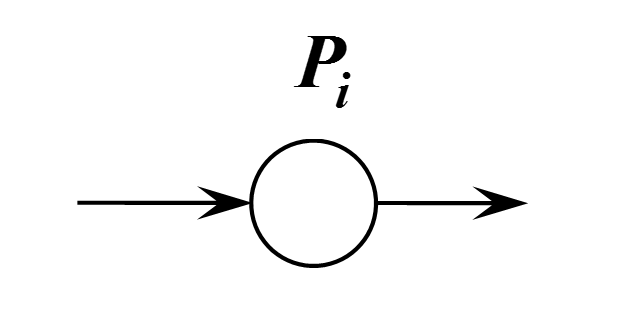
\includegraphics[width=0.7\textwidth]{place} \\ а)}
	  	\end{minipage}
	  	\hfill
	  	\begin{minipage}[ht]{0.49\linewidth}
	  		\center{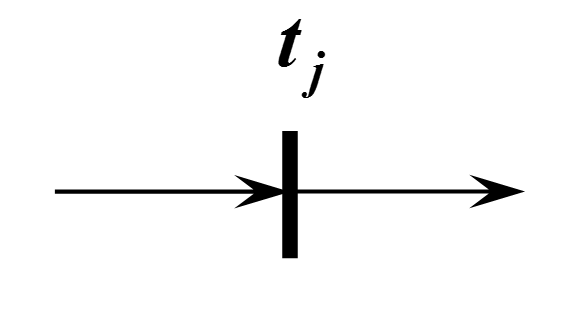
\includegraphics[width=0.8\linewidth]{tansition} \\ б)}
	  	\end{minipage}
	  	\caption{a) "--- изображение позиции, б) "--- изображение перехода. }
	  	\label{img:example}  
	  \end{figure}
	  
	  Ориентированные дуги могут соединять только позиции и переходы в прямом и обратном направлении (свойство двудольности~\cite{piterson}). Сеть Петри является мультиграфом, так как допускается кратность дуг между позициями и переходами (вершинами графа). Пример сети Петри приведен на рисунке \ref{img:petri-net}
	  
	  	\begin{figure}[h!]
	  		\center{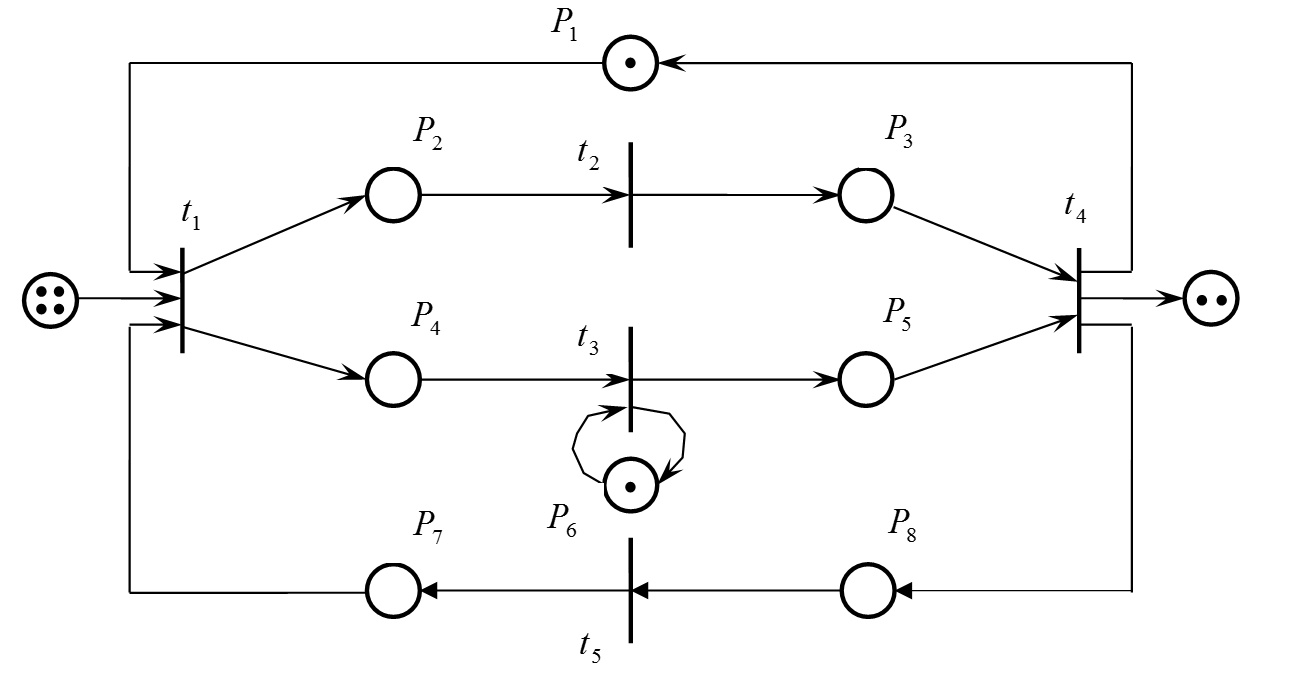
\includegraphics[width=0.7\textwidth]{petri-net}}
	  		\caption{Пример сети петри.}
	  		\label{img:petri-net}
	  	\end{figure}
	  
	  Сетью Петри принято называть тройку $<G, m_0,\rho>$  , где  $G\equiv<P,T,I,O>$ "--- граф сети Петри, $P$   "--- конечное множество позиций (или мест) сети, $T$ "--- конечное множество переходов сети, $P \cap T = \varnothing$. $I,O:T\rightarrow P^{()}$  "--- функции, задающие комплекты входных и, соответственно, выходных позиций переходов сети (здесь $P^{()}$  "--- множество всевозможных конечных комплектов элементов множества $P$ ). $M \cong P^{()}$ "--- множество всевозможных состояний сети (маркировок).  $m_0 \in M$ "--- начальная маркировка сети, задающая начальное состояние сети, $\rho:T\rightarrow C$ "--- функция раскраски, возможно частичная, где $C$  "--- множество красок.
	  
	  Сеть называется ограниченной, если $ (\forall p \in P) (\exists k \in \textit{nat}) (\forall m \in \mu_0) (m(p) \leq k)$, то есть множество достижимых в сети маркировок конечно.
	  
	Ограниченная сеть Петри $S$ на множестве позиций $P$, $|P|\in \aleph_0$, может быть представлена следующим образом~\cite{falkTheory}:\\ 
	$ S \subseteq P^{()} \times (P^{()} \times P^{()}) $
	
	Неограниченная сеть Петри $S$ на  $P$, $|P|\in \aleph_0$:	$ S \subseteq P^{()} \times 2^{P^{()} \times P^{()}} $
	
	Для любой сети Петри $S\equiv < m_0, T >,\;  m_0 \in P^{()}$ называется начальной разметкой сети, а направленное квазиотношение $T$ -- множество переходов сети.
	
	Сети Петри рассматриваются с точностью до изоморфизма: две сети $S'\equiv<{m'}_0, T'>$ на $P'$ и $S''\equiv<{m''}_0, T''>$ на $P''$ изоморфны ($ S' \sim S'' $), если существует взаимооднозначное соответствие $ \varepsilon:P'\leftrightarrow P'' $, такое, что $ \varepsilon(T') = T'' $. Графическое представление сетей Петри хорошо известно и не нуждается в уточнении.
	
	Бинарное отношение $\mathrm{T}(T)$ изменения разметок на множестве $P^{()}$ разметок сети Петри $S\equiv < m_0, T >$:
	\begin{center}
		$\mathrm{T}(T)\cong\{<p',p''-p_1+p_2>|<p_1,p_2> \in T \wedge p_1\leq p''\}$
	\end{center}

	История поведения стандартной ограниченной сети Петри $S\equiv < m_0, T >$: кортеж $<m_0,m_1,...,m_k>$, 
	такой, что $(\forall i \in 1..k)(<m_{i-1}, m_i> \in \mathrm{T}(T))$
	
	Множество всех возможных историй поведения сети Петри $S$ обозначим $\mu(S)$.
	
	Две сети Петри $S_1$ и $S_2$ эквивалентны, если $\mu(S_1) \sim \mu(S_2)$ (т.е. существует взаимно-однозначное соответствие $\varepsilon:P'\leftrightarrow P''$, такое, что $\varepsilon(\mu(S')) = \mu(S'')$)
	
  \subsection{Сети Петри со строгой дисциплиной изменения разметок}
	Бинарное отношение $\bar{\mathrm{T}}(T)$ строгого изменения разметок на множестве $P^{()}$ 
	разметок сети в сети Петри $S\equiv < m_0, T >$~\cite{falkTheory}:
	\begin{equation}
		\begin{multlined}
			\bar{\mathrm{T}}(T)\cong\{<p',p''-p_1+p_2>|<p_1,p_2> \in T \wedge p_1\leq p'' \wedge\\
			\wedge (\exists<{p'}_1, {p''}_2> \in T)(p_1 < {p'}_1 \wedge {p'}_1 \leq p'') \}
		\end{multlined}
	\end{equation}
	  
	История поведения ограниченной сети Петри $S\equiv < m_0, T >$ со строгим изменением разметок: кортеж  $<m_0,m_1,...,m_k>$, 
	такой, что\\ $(\forall i \in 1..k)(<m_{i-1}, m_i> \in \bar{\mathrm{T}}(T))$
	  
	Пусть задана стандартная ограниченная сеть Петри $S\equiv < m_0, T >$. Пополним множество $P$ ее позиций множеством $P_G$ новых элементов,
	взаимно-однозначно соответствующих переходам из $G$: $P'\cong P\cup P_G$,\\ 
	$P_G\cong \{p_t|(t\in T)\wedge (p_t \notin P)\}$. Искомую ограниченную сеть Петри со строгой дисциплиной изменения разметок 
	обозначим $S'\equiv  < {m'}_0, T >$:\\
	${m'}_0\cong m_0 +\displaystyle\sum_{p_t\in P_G}c_{p_t}$,
	$T'\cong\{\alpha'+c_{p_{<\alpha',\alpha''>}}, \alpha'' +c_{<p_{\alpha',\alpha''>}}|<\alpha',\alpha''> \in T\} $.
	Доказательство эквивалентности сетей $S$ и $S'$ очевидно.
  \subsection{Динамические вычислительные сети}
	 % Для отображения символа в большом варианте использовать \displaystyle
	Пусть 
	$ D = \displaystyle\bigcup_{\theta\in\Theta} D_\theta $  - многосортный \textit{универсум данных},  
	где $\Theta$ - конечное множество \textit{сортов} данных, 
	$D_\theta$ - подмножество \textit{данных} сорта $\theta\in\Theta$.\\
	Будем считать, что одним из таких сортов данных является сорт \textit{nat}, такой, что $D_{\textit{nat}} \cong \aleph_0$.
	Функциональным базисом будем называть конечное множество  $ B $   всюду определенных вычислимых~\cite{falkTheory} функций вида:\\
	$ \beta: \displaystyle\bigtimes_{i'\in 1..m'}D_{\theta'_{i'}} \rightarrow \displaystyle\bigtimes_{i''\in 1..m''}D_{\theta''_{i''}} $, $ m',m'' \in \aleph_0 $  , 
	где  $ <m',m''> $   называется арностью функции $ \beta $  , а  $ <\nu',\nu''> $  , $ \nu'\in \Theta^{<m'>}, \nu''\in \Theta^{m''}  $ -- ее типом.
	\subsubsection{Определение}
		\textit{ Динамической вычислительной сетью} (\textbf{ДВС}) в функциональном базисе $B$ 
		назовем пару $<\bar{\Sigma},\dot{S}>$, где $\overline{\Sigma}$ 
		- конечное множество классов сетей ДВС, $\dot{S}$ - аксиома ДВС.
		 
		Каждый класс $\Sigma$ характеризуется: 
		уникальным именем  $\dot{\Sigma}$, 
		типом функции 
		$< |\bar{\theta}'(\dot{\Sigma})|,|\bar{\theta}''(\dot{\Sigma})|>$
		,  и конечным упорядоченным множеством $S^*(\dot{\Sigma})$
		\textit{образов сетей} этого класса.
		Тип или арность может указываться,
		при необходимости, в виде правого верхнего индекса.
		 
		Все образцы сетей из $S^*(\dot{\Sigma})$ имеют тот же тип, а, следовательно,
		и арность, что и сам класс $\Sigma$.
		Тип или арность образца сети   $S\in\bar{S}(\dot{\Sigma})$ ,
		при необходимости, также может указываться в виде его правого верхнего индекса.
		 
		Образец сети  $S\in{S^*(\dot{\Sigma})}$   в общем случае имеет вид:
		\begin{center}
			$S\cong<P,\delta,I,O,T_T,T_H,\nu',\nu'',I_T,O_T,\sigma,\rho,\varphi_T,\lambda_I,\lambda_O,\mu_0> $,где
		\end{center}
		\begin{itemize}
		  \item $P$ 
		  "--- конечное множество элементов\footnote{Используемый здесь термин «элемент сети» является, во-многом, аналогом терминов «позиция» или «место» в теории сетей Петри и «точка сети» в теории направленных отношений.}
		    образца сети,
		 
		  \item $\delta:P \rightarrow \Theta$  "--- задает сорта элементов образца сети,
		  \item  $I,O \in P^{<>}$ "--- кортежи входных и выходных элементов образца сети, \mbox{$<\delta(I),\delta(O)>$}  "---  тип, а $<|I|,|O|>$   "--- арность образца сети,
		  
		  \item $T_T$ 
		  "--- конечное множество терминальных переходов,
		  
		  \item $T_H$ 
		  "--- конечное множество нетерминальных переходов,
		    $T_T \cap T_H = \varnothing$  , $T\cong  T_T \cup T_H$ , $T \cap P = \varnothing$ ,
		 
		  \item	для всех $ t \in T$  : $I_T(t) \in P^{<\nu'(t)>}$ ,
		   $ O_T(t) \in P^{\nu''(t)} $  ;\\
		    $<\nu'(t), \nu''(t)>$   "--- \textit{арность перехода}  $ t \in T $   ( $ \nu',\nu'':T\rightarrow\aleph_0 $ ),\\
		  $ <\delta(I_T(t)),\delta(O_T(t))> $  "--- \textit{тип перехода} $t$  , 
		  
		  \item $ \sigma:T_H \rightarrow \{ \dot{\Sigma}\;| \;\Sigma \in \bar{\Sigma} \} $ (сопоставляет имена классов сетей-объектов нетерминальным переходам),
		  
		  \item $ \rho:T_H \rightarrow \Re_0 $ (задает \textit{временные сдвиги} для нетерминальных переходов),
		  
		  \item $ \omega:T_H \rightarrow P $(задает \textit{управляющие входы} нетерминальных переходов), для всех  $ t \in T_H $  $ \delta(\omega(t)) = \textit{nat} $   ;
		  
		  \item $ \varphi_T:T_T \rightarrow B $ – \textit{семантика} терминальных переходов, причем для всех  $ t \in T_T $    тип  $\varphi_T(t)$    равен  $ <\delta(I_T(t)),\delta(O_T(t))> $  ,
		  
		  \item $ \lambda_I:\{ <t,i'>|\;t\in T_T \wedge i' \in 1..\nu'(t) \} \rightarrow \Re_0 $ и
		  
		  \item $ \lambda_O:\{ <t,i''>|\;t\in T_T \wedge i'' \in 1..\nu''(t) \} \rightarrow \Re_0 $ задают «задержки» входных и выходных связей терминальных переходов с элементами образца сети,
		  
		  \item $ \mu_0 \in M_S $ , 
		  где $ M_S \cong \{ \mu\;|\; (\forall p \in P)(\mu(p) \in (D_{\delta(p)} \times \Re_0)^{()} \} $.
		  Компонент $ \mu_0 $    является, в определенном смысле, аналогом понятия маркировки сетей Петри,
		  в связи с чем множество  $ M_S $   будем тоже называть \textit{множеством возможных маркировок} сети,
		  а $\mu_0$   – ее \textit{начальной маркировкой}.
		  Не ограничивая общности, далее будем считать, что для любой маркировки  $\mu\in M_S$
		  все комплекты  $\mu(p)$  (для всех $p \in P$ ) представлены кортежами вида 
		  $ < <d_1,\tau_1>,...,<d_{|\mu(p)|}, \tau_{|\mu(p)|} > $  , 
		  построенными из элементов соответствующего комплекта так, 
		  что компоненты кортежей упорядочены по неубыванию вторых компонентов пар 
		  (т.е. $ (\forall i\in 1..|\mu|-1) (\tau_i \leq \tau_{i+1}) $~). 
		\end{itemize}
		 
		 \newtheorem{com}{Замечание}
		 \begin{com}\label{izomorph}
		 		Заметим, что образцы сетей рассматриваются с точностью до $(P, T_T, T_H)$-изоморфизма.
		 \end{com}
		 
		\textit{ Аксиома} или, по-иному, инициальное состояние $\dot{S}$ ДВС (корень дерева состояний) -- один из образцов некоторого класса $\Sigma \in \bar{\Sigma}$.
	\subsubsection{Графическое представление ДВС}
		Графическое представление ДВС опишем как совокупность графических представлений множества $\bar{\Sigma}$ классов 
		и сети $\dot{S}$ - аксиомы ДВС (рисунок \ref{img:DNC-graphic})
		\begin{figure}[h!]
			\center{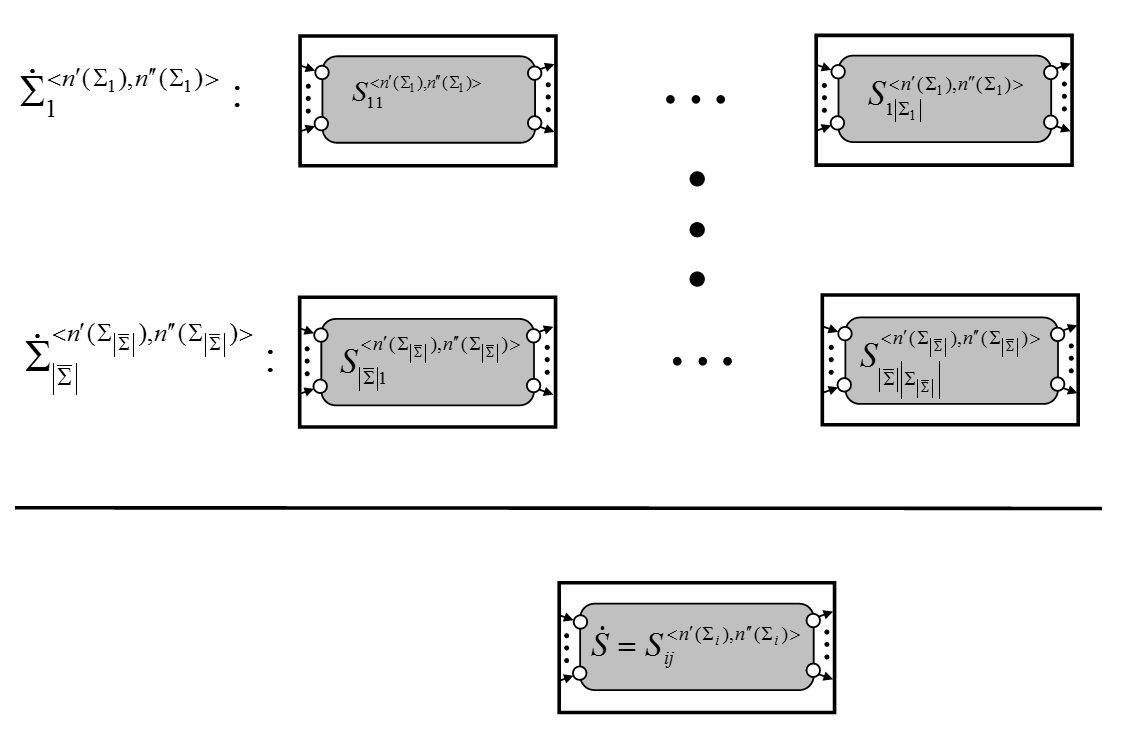
\includegraphics[width=0.8\textwidth]{DNC-graphic}}
			\caption{Графическое представление ДВС.}
			\label{img:DNC-graphic}
		\end{figure}
		
		\begin{figure}[h!]
			\begin{minipage}[ht]{0.49\linewidth}
				\center{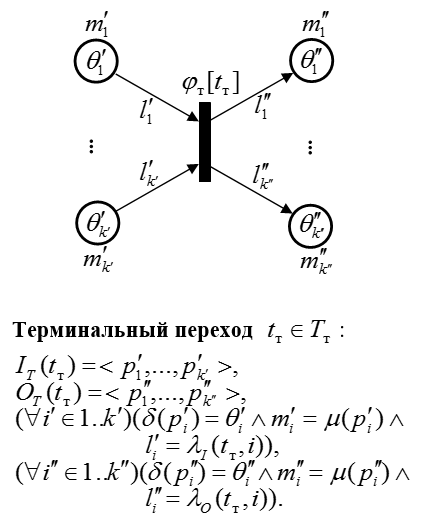
\includegraphics[width=0.8\linewidth]{terminal-t} \\ а)}
			\end{minipage}
			\hfill
			\begin{minipage}[ht]{0.49\linewidth}
				\center{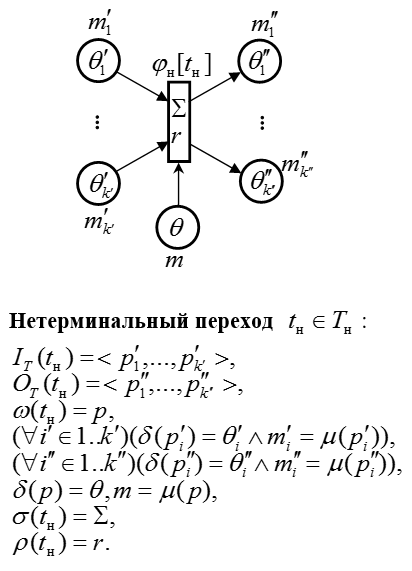
\includegraphics[width=0.8\linewidth]{non-terminal-t} \\ б)}
			\end{minipage}
			\caption{Графическое представление компонентов сетей.}
			\label{img:components}  
		\end{figure}
		
		Графическое представление класса $\Sigma$ включает имя $\dot{\Sigma}$ этого класса 
		и множество графических представлений образцов сетей этого класса. За основу представления сетей (образцов сетей) 
		взято представление сетей отношений в теории направленных отношений, представление элементов сети и переходов 
		фактически заимствовано из наиболее часто используемых представлений позиций и переходов сетей Петри 
		и их различных расширений и модификаций, а прочие компоненты в графическом представлении указываются 
		в качестве меток элементов графических представлений рассмотренных выше компонентов на рисунке \ref{img:components}.
		представлены представления терминальных и нетерминальных переходов, включая связанные с ними входные и выходные элементы сети.
		%Рис 4. %TODO вставить ссылку на рисунок
		%содержит пример представления ДВС.

	
	\subsubsection{Процесс в ДВС}
		\textit{Процесс} в ДВС -- прадерево смены состояний ДВС (далее -- дерево состояний). Дерево состояний строится на основе определения готовности к срабатыванию терминальных и нетерминальных переходов и определения нового состояния ДВС в результате срабатывания некоторого перехода из числа готовых к срабатыванию согласно правилу выбора перехода.
		За основу этого правила принята описанная выше строгая дисциплина срабатывания переходов, уточнение которой приведено ниже. Если согласно этой дисциплине возможно срабатывание нескольких переходов, то срабатывание каждого из них определяет свою ветвь в дереве состояний.
	
	\paragraph{Правило выбора переходов}

		Пусть $ S\cong<P,\delta,I,O,T_T,T_H,\nu',\nu'',I_T,O_T,\sigma,\rho,\varphi_T,\lambda_I, \lambda_O,\mu> $
		-- текущее состояние ДВС.  Готовность к срабатыванию переходов в любые моменты времени определяется значением
		предиката $ U:T\times\Re_0\rightarrow\{true,false\} $.
		
		Для определения значения $ U(t,\tau) $    для терминальных переходов $t\in T_T$
		введем вспомогательный предикат  $ {U^{i,l}_T} $     
		с двумя параметрами $ i\in \aleph_0 $   и $ l:P\rightarrow\aleph_0 $  .
		Для  $ t\in T_T $   положим $ U(t,\tau)\cong {U^{1,l_0}}_T(t,\tau) $  ,
		где $ (\forall p\in P)(l_0(p) = 0) $  , и $ I_T(t)=<{p_1}',...,{p_{\nu'(t)}}' > $   .
		Тогда 
		\begin{equation}
			{U^{i,l}}_T(t,\tau)\cong
			\begin{cases}
				true, \quad \text{если}\; i > \nu'(t),\\
				U^{i+1,l'}_T(t,\tau)\wedge(l(p_i')\leq|\mu(p_i')|)\wedge(\mu(p_i')(l(p_i')) (2) +\lambda_I(t,i)\leq \tau),\\
				\quad \text{где } l'(p_i')=l(p_i')+1, (\forall p \not= p_i')(l'(p_i')=l(p_i'), \quad \text{если } i\leq \nu'(t)
			\end{cases}
		\end{equation}
		
		Если   $ t\in T_H $ , то	
		\begin{equation}
			U(t,\tau)\cong(|\mu(\omega(t))|>0)\wedge(head(\mu(\omega(t)))(2)\leq \tau).
		\end{equation}
		
		Переход  $ t\in T $   может сработать в момент времени  $ \tau\in\Re_0 $   и образовать свою ветвь в дереве состояний,
		если он готов к срабатыванию и нет готовых к срабатыванию в тот же момент времени более приоритетных переходов.
		Используемая строгая дисциплина срабатывания переходов предполагает, 
		что переход $ t\in T $ имеет более высокий приоритет, чем переход  $ t'\in T $  ,
		если $ (\forall\mu \in M_S)(\forall \tau \in \Re_0) (U(t,\tau)\supset U(t',\tau) $  .
		
		Наконец, определим новое состояние ДВС, находившейся в состоянии $ S $  , 
		после срабатывания в момент времени   $ \tau \in \Re_0 $  некоторого перехода. 
		Отдельно рассмотрим случай  $ t\in T_T $   и случай  $ t\in T_H $ . 
		Обозначим новое состояние в результате срабатывания этого перехода как  $ \vec{S} $ . 
		Пусть $ \tau $   -- минимально возможное время, в которое может сработать какой-то переход $ t\in T $  .
		\begin{enumerate}
			\item Если  $ t\in T_T $ , то
			$ \vec{S}\cong<P,\delta,I,O,T_T,T_H,\nu',\nu'',I_T,O_T,\sigma,\rho,\varphi_T,\lambda_I,\lambda_O,\vec{\mu} >$, 
			где новая маркировка $ \vec{\mu} $  определяется выполнением следующего алгоритма, использующего, 
			помимо параметра цикла $ i:\aleph_0$\footnote{Запись $x:\chi$ означает, что программная переменная $x$ имеет область значений $\chi$}   и вспомогательной переменной $ p:P $  , 
			две «переменные»  $ arg:\displaystyle\bigtimes_{i'\in 1..\nu'(t)}D_{\delta(p_{i'}')} $, 
			$ val: \displaystyle\bigtimes_{i''\in 1..\nu''(t)} D_{\delta(p_{i''}'')} $  
			для хранения, соответственно, значения аргумента и значения функции $ \varphi_T $  , представляющей семантику терминального перехода:\\
			
			\begin{minipage}[ht]{0.8\textwidth}
	\begin{algorithm}[H]
		\Begin
		{
			$\bar{\mu}:=\mu$;\\
			$i:=1 $;\\
			$ arg:=<> $;\\
			\While{$ i\leq \nu'(t) $}
			{
				$ p:=I_T(t)(i) $;\\
				$ arg:=arg<head(\vec{\mu}(p))(1)> $;\\
				$ \vec{\mu}(p):=tail(\mu(p)) $;\\
				$ i:=i+1 $;\\	
			}
			$ val:=\phi_T(t)(arg) $;\\
			$ i:=1 $;\\
			\While{$ val\not=<> $}
			{
				$ p:=O_T(t)(i) $;\\
				$ \vec{\mu}(p):=\vec{\mu}(p)+1_{<head(val),\tau+\lambda_O(<t,O_T(t)(i)>) } $;\\
				$ val:=tail(val) $
			}
		}
		
		\caption{Алгоритм нахождения маркировки.}
	\end{algorithm}
\end{minipage}

			\item Если $ t\in T_H $  , $ p=\omega(t) $ , то сеть $ \vec{S} $    
			будет получена подстановкой сдвинутого во времени образца сети  $ S^*(\sigma(t))[head(\mu(p))(1)] $   
			(с начальной маркировкой  $ \bar{\mu}_0 $ ) в сеть $ S $    вместо нетерминального перехода $ t $ , 
			с предварительным удалением «головного» элемента из кортежа $ \mu(p) $: $ \mu(p):=tail(\mu(p)) $ .
		\end{enumerate}
	\paragraph{Срабатывание перехода}		
		Пусть  $ \bar{S}\equiv<\bar{P},\bar{\delta},\bar{I},\bar{O},
		\bar{T}_T,\bar{T}_H,\bar{\nu}',\bar{\nu}'',\bar{I}_T,\bar{O}_T,\bar{\sigma},
		\bar{\rho},\bar{\varphi}_T,\bar{\lambda}_I,\bar{\lambda}_O,\bar{\mu}> $ , где все компоненты $ \bar{S} $   , кроме $ \bar{\mu} $  ,
		взяты из упомянутого образца сети, а сдвиг во времени означает, что для всех  $ p\in \bar{P} $ ,  
		если \( \bar{\mu}_0(p)=<<d_1,\tau_1>,...,<d_k,\tau_k>>\) , то $ \bar{\mu}(p)=<<d_1,\tau_1+(\tau+\rho(t))>,...,<d_k,\tau_k+(\tau+\rho(t))>> $  , 
		т.е. вторые компоненты элементов начальной маркировки в подставляемом образце интерпретируются как временные интервалы 
		относительно момента времени его срабатывания, сдвинутые дополнительно индивидуально для конкретного нетерминального перехода. 
		
		Результат  $ \vec{S} $    подстановки сети   $ \bar{S} $   в сеть   $ S $  вместо ее нетерминального перехода  $ t\in T_H $   
		определяется во многом аналогично тому, как определена операция подстановки для сетевых представлений направленных отношений.
		
		Согласно \textit{Замечанию~\ref{izomorph}} будем считать, что 
		$ P\cap\bar{P} = \emptyset $, 
		$ T_T\cap\bar{T}_T=\emptyset $, 
		$ T_H\cap \bar{T}_H=\emptyset $.
		Определим отношение эквивалентности, обозначаемое инфиксом $ \approx $ , как рефлексивное, симметричное, транзитивное замыкание бинарного отношения 
		$ \{ <I_T(t)(i),\bar{I}(i)>|i\in 1..\nu'(t) \} \cup \{<O_T(t)(i),\bar{O}(i)>|i \in 1..\nu''(t) \} $. 
		Множество элементов полученной в результате подстановки сети определим как фактор множества  $ P\cap\bar{P} $  по отношению  $ \approx : \vec{P}\cong(P\cup\bar{P})\;/\approx$, 
		а для определения всех остальных компонентов  $ \vec{S} $  (функции рассматриваются как графики) произведем в покомпонентном объединении сетей  $ S $   и $ \bar{S} $   
		замену элементов из $ P\cup\bar{P} $ на соответствующие элементы из  $ \vec{P} $  (на классы эквивалентности, в которые они входят):\\
		\begin{equation}
		\begin{multlined}
		\vec{S}\cong[(\forall p \in P \cup \bar{P} )(p\Rightarrow(p\; / \approx) )] 
		<P\cup\bar{P},\delta\cup\bar{\delta},I\cup\bar{I},O\cup\bar{O},T_T\cup\bar{T}_T,\\
		T_H\cup\bar{T}_H,\nu'\cup\bar{\nu}',\nu''\cup\bar{\nu}'',I_T\cup\bar{I}_T,
		O_T\cup\bar{O}_T,\sigma\cup\bar{\sigma},\rho\cup\bar{\rho},\varphi_T\cup\bar{\varphi}_T,
		\lambda_I\cup\bar{\lambda}_I,\\
		\lambda_O\cup\bar{\lambda}_O,\mu\cup\bar{\mu}>
		\end{multlined}
		\end{equation}
		
		Для выполнения операции замены в объединении графиков функций, 
		область определения которых пересекается с областью  $ P\cup\bar{P} $  объектов замены, требуется уточнение. 
		Для случая $ [(\forall p \in P \cup \bar{P} )(p\Rightarrow(p\; / \approx) )](\delta\cup\bar{\delta})$   
		проблем не возникает, и можно воспользоваться общим правилом:\\
		$[(\forall p \in P \cup \bar{P} )(p\Rightarrow(p\; / \approx) )](\delta\cup\bar{\delta}) \cong
		[(\forall p \in P \cup \bar{P} )(p\Rightarrow(p\; / \approx) )] \delta \cup [(\forall p \in P \cup \bar{P} )(p\Rightarrow(p\; / \approx) )]\bar{\delta}$,\\
		так как в результате объединения результатов замены получится функциональный график, 
		а для случая  $ [(\forall p \in P \cup \bar{P} )(p\Rightarrow(p\; / \approx) )](\mu\cup\bar{\mu}) $   
		в результате объединения результатов замены график может оказаться не функциональным. 
		Поэтому для случая, когда замена осуществляется в графике функции с областью определения  $ P\cup\bar{P} $  
		и значениями-комплектами из множеств  $ (D_{\delta(p)}\times\Re_0) $  для всех $ p\in P\cup \bar{P} $, 
		результат замены определим по иному:\\
		$ [(\forall p \in P \cup \bar{P} )(p\Rightarrow(p\; / \approx) )](\mu\cup\bar{\mu})\cong
		\{<p',\!\displaystyle\sum_{p \in (p'/\approx)}\!(\mu\cup\bar{\mu})(p)| p' \in ((P\cup\bar{P}) /\!\approx) \} $.
		
   \subsubsection{Сборка <<мусора>>  в ДВС}
	   Мусором в состояниях-вершинах дерева состояний ДВС мы будем называть 
	   \begin{enumerate}
		   \item переходы состояния, которые заведомо не смогут сработать ни в одном из подчиненных состояний, т.е. в других состояниях, к которым из этого состояния есть путь в дереве состояний,
		   \item элементы состояний, используемые во всех подчиненных состояниях исключительно как входные и выходные элементы исключаемых «мусорных» переходов.
	   \end{enumerate}

	   Мусор исключается из всех подчиненных состояний того состояния в дереве, в котором для перехода или для элемента установлен статус «мусора».
	   
	   Алгоритм выявления мусора во многом подобен алгоритму сборки мусора при выполнении программ в большинстве реализаций языков программирования. Он предполагает выполнение следующих шагов:
	   \begin{enumerate}
		   \item первоначально все переходы и элементы сети полагаются мусорными;
		   \item отмечаем как немусорные переходы, все входные элементы которых имеют непустую маркировку (в том числе и переходы с пустым кортежем входных позиций),  либо отмечены как немусорные;
		   \item отмечаем как немусорные элементы, являющиеся выходными для не-мусорных переходов;
		   \item повторяем шаги 2 и 3 до тех пор, пока при их выполнении отмечается как немусорный хотя бы еще один новый переход или элемент.
	   \end{enumerate}
	   
	   Оставшиеся переходы, не отмеченные как немусорные, удаляются из сети, вместе с элементами ассоциированных с ними графиков функций. %Оставшиеся элементы, не отмеченные как немусорные, ...
	
	\section{Предметно-ориентированные языки и их реализация в Meta Programing System}
		\subsection{Структура языка}

		Проектирование языка начинается с определения структуры языка.~\cite{mpssource}
		
		Абстрактное синтаксическое дерево (англ. Abstract Syntax Tree) - логическое представление кода в памяти в виде дерева, который описывает иерархию узлов. Эти узлы имеют понятие отношений родитель-ребенок. Кроме того, два узла могут быть соединены друг с другом с явными ссылками, которые идут по всей иерархической структуре.
		
		\begin{figure}[ht] 
			\centering
			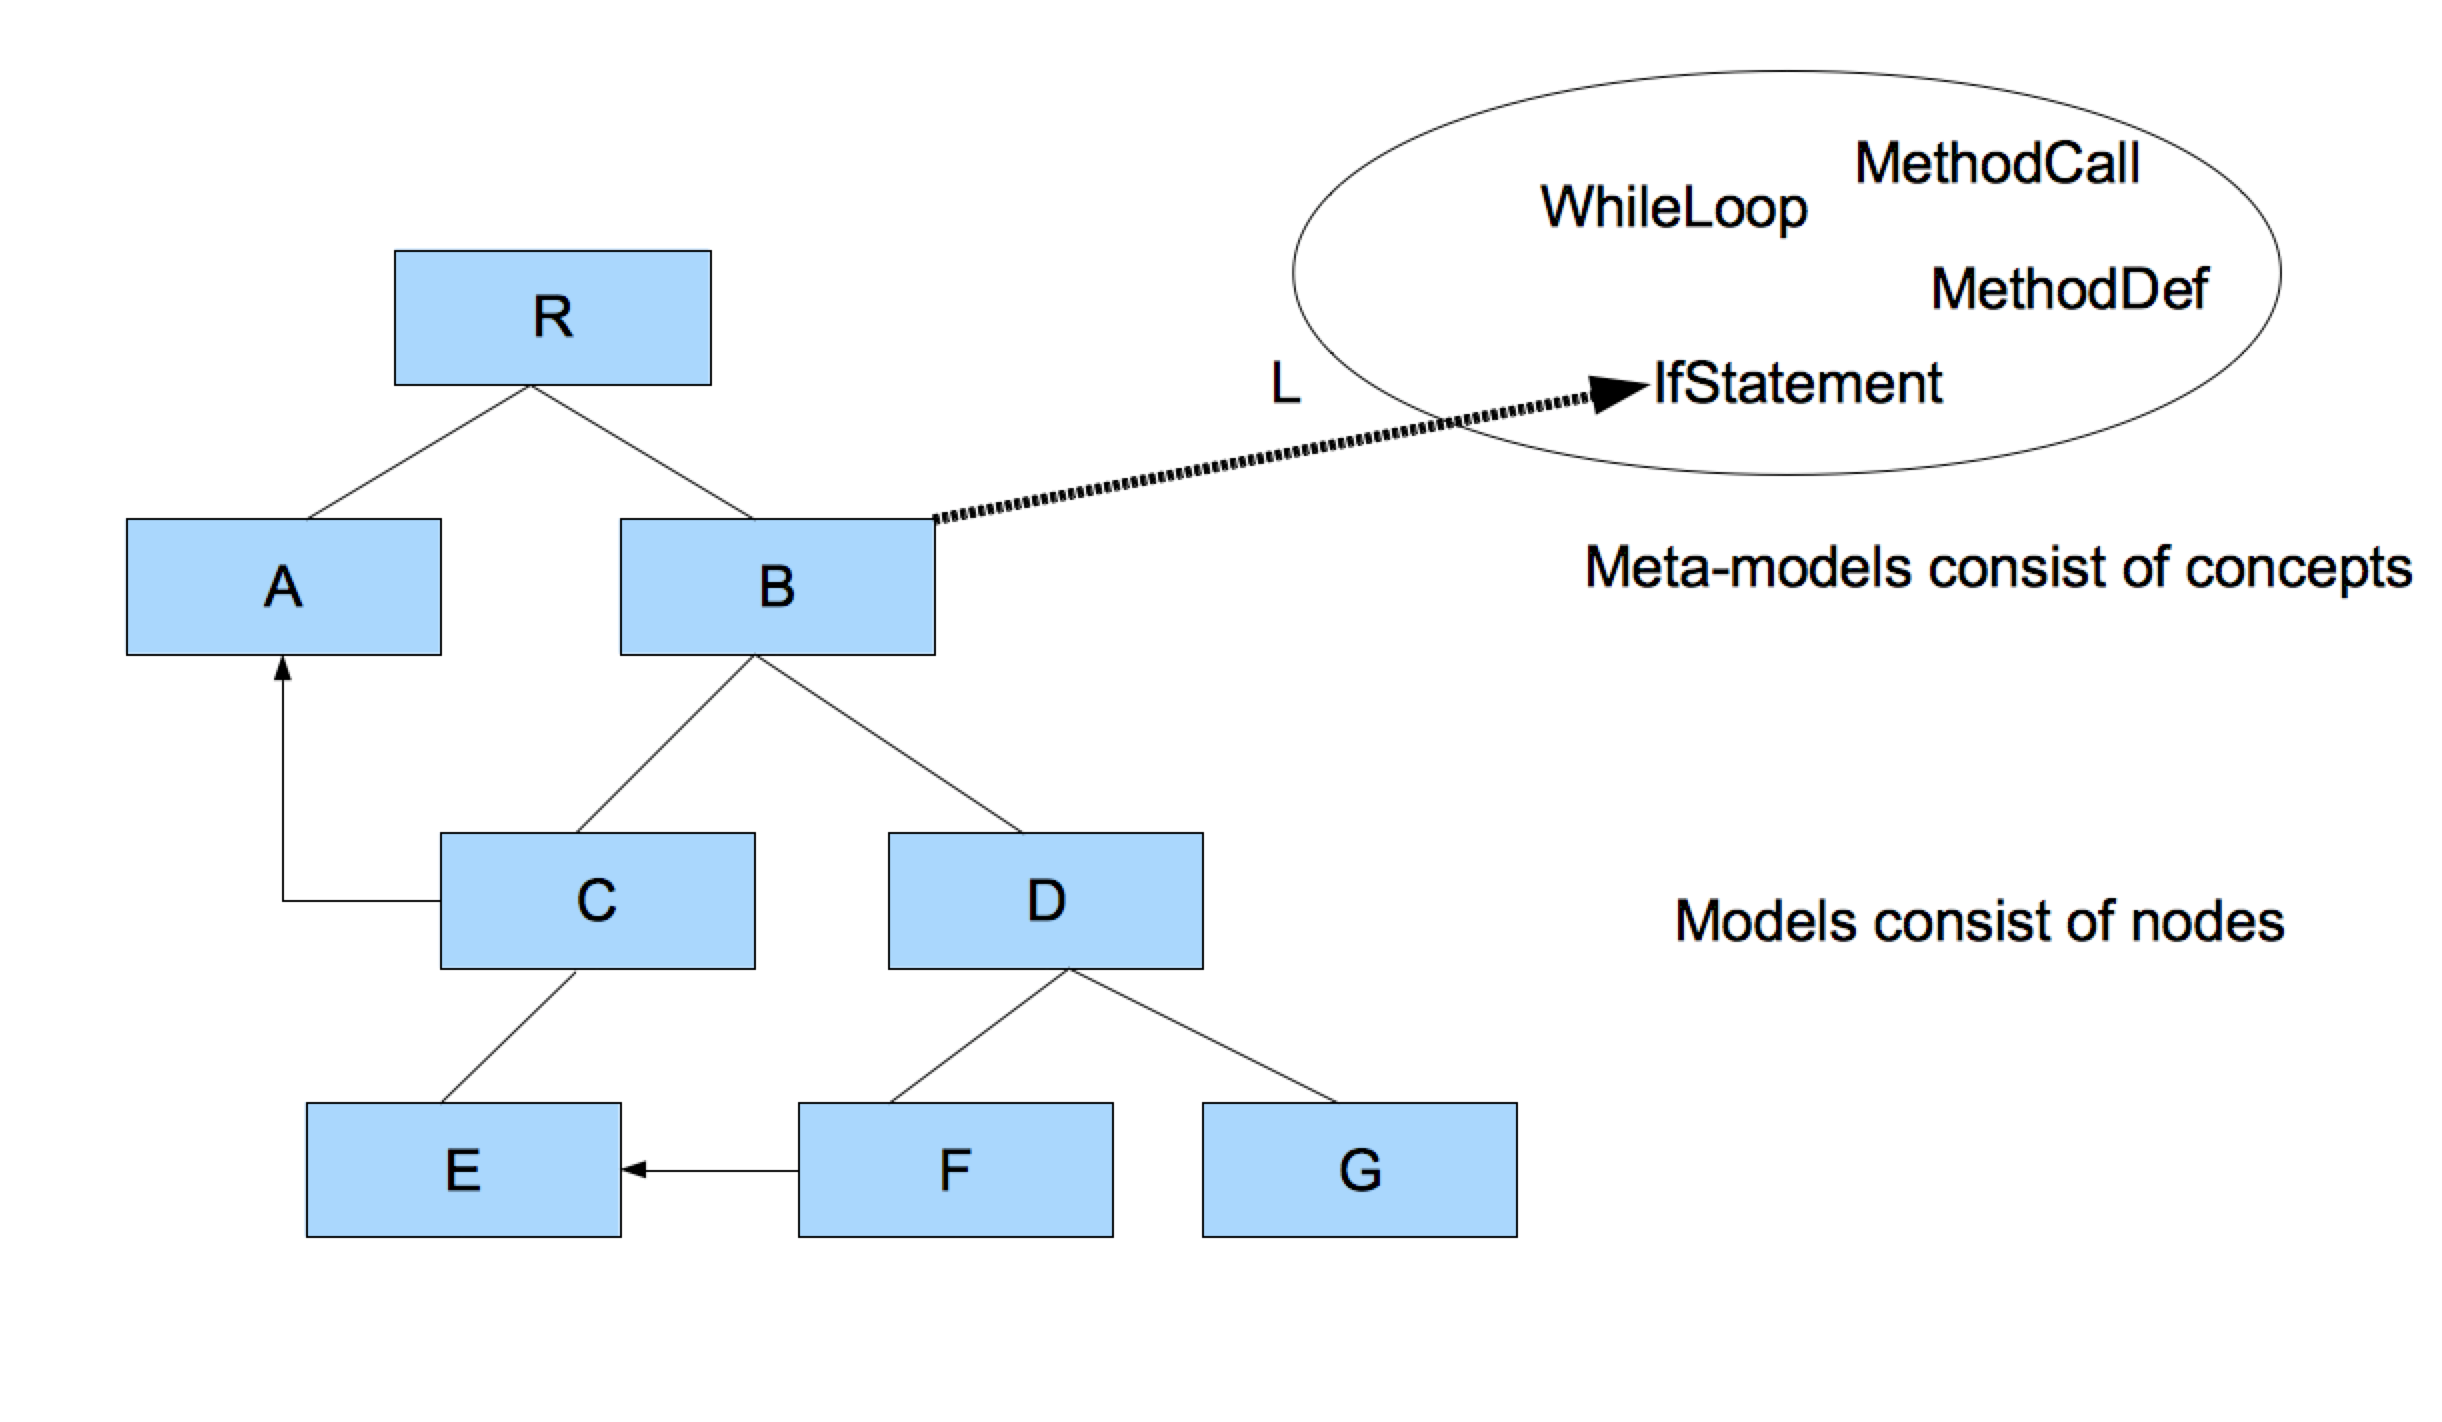
\includegraphics [scale=0.27] {AST}
			\caption{Абстрактное синтаксическое дерево} 
			\label{img:AST}  
		\end{figure}
	
		АСД-узлы организованы в модели. Узлы, которые не имеют родителей, называются корневыми узлами. Это элементы языка, лежащие на самом верхнем уровне. Например, в языке Java корневые узлы -- классы, интерфейсы и перечислимые типы.
		
		Узлы могут сильно отличаться друг от друга. Каждый узел сохраняет ссылку на своё определение -- концепцию. Концепция определяет тип узлов и задаёт структуру узлов данного класса. Она определяет, какие дети, свойства и ссылки может иметь экземпляр узла. Определения концепции формируются в объектно-ориентированной парадигме. Если одна концепция расширяет другую, она наследует всех детей, свойства и ссылки от своего родителя.
		
		\subsubsection{Определение концепции в MPS}
		
			В MPS для определения концепции используется встроенный язык Structure Language.~\cite{mpssource} Пример определения концепции можно увидеть на рис. \ref{img:concept1}.
			
			\begin{figure}[ht] 
				\center
				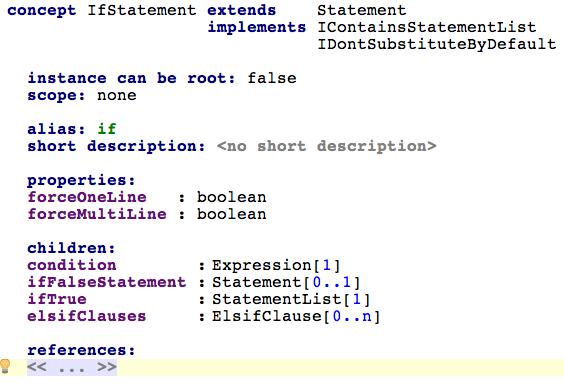
\includegraphics [scale=0.7] {concept1}
				\caption{Пример определения концепции} 
				\label{img:concept1}  
			\end{figure}
		
		Концепции имеют 2 типа наследования: расширение имеющейся концепции и реализация концептуального интерфейса. 
		
		Свойства концепции определяются после ключевого слова \textbf{properties}. Свойство представляет собой значение, которое хранится внутри экземпляра концепции. Каждое свойство должно иметь тип, который для свойств ограничен до: примитивов, таких как булевый тип, строка и целое; перечислений, которые могут иметь значение из заранее заданного набора; и ограниченных типов данных (строк, ограниченных регулярными выражениями).
		
		Ссылки определяются после ключевого слова \textbf{references}. Для повышения выразительности языков узлам разрешено хранить ссылки на другие узлы. Каждая ссылка имеет имя, тип, и количество элементов (мощность). Тип ограничивает допустимый типом цели ссылки. Мощность определяет, как много ссылок такого рода узел может иметь. Ссылки могут только два типа мощностей: $ 1:0..1 $ и $ 1: 1$.
		
		Дети определяются после ключевого слова \textbf{children}. Каждое определение ребенок держит целевую концепцию, ее роль и количество элементов. Целевая концепция определяет тип детей. Роль определяет имя для этой группы детей. И, наконец, количество элементов определяет, сколько детей из этой группы могут содержаться в одном узле. Есть 4 разрешенных вида мощности: $ 1: 1 $, $ 1: 0..1 $, $ 1: 0..n $ и $ 1: 1..n $.
		
		Поле \textbf{alias} задаёт строку, с которой MPS будет ассоциировать данную концепцию.
		
	\subsection{Ограничения}
		Структуры языка иногда может быть недостаточно, чтобы выразить дополнительные ограничения. MPS содержит возможность задать для каждой концепции определить такие дополнительные ограничения в пакете, под названием \textit{Constraints}.~\cite{mpssource}
		
		\begin{figure}[ht] 
			\center
			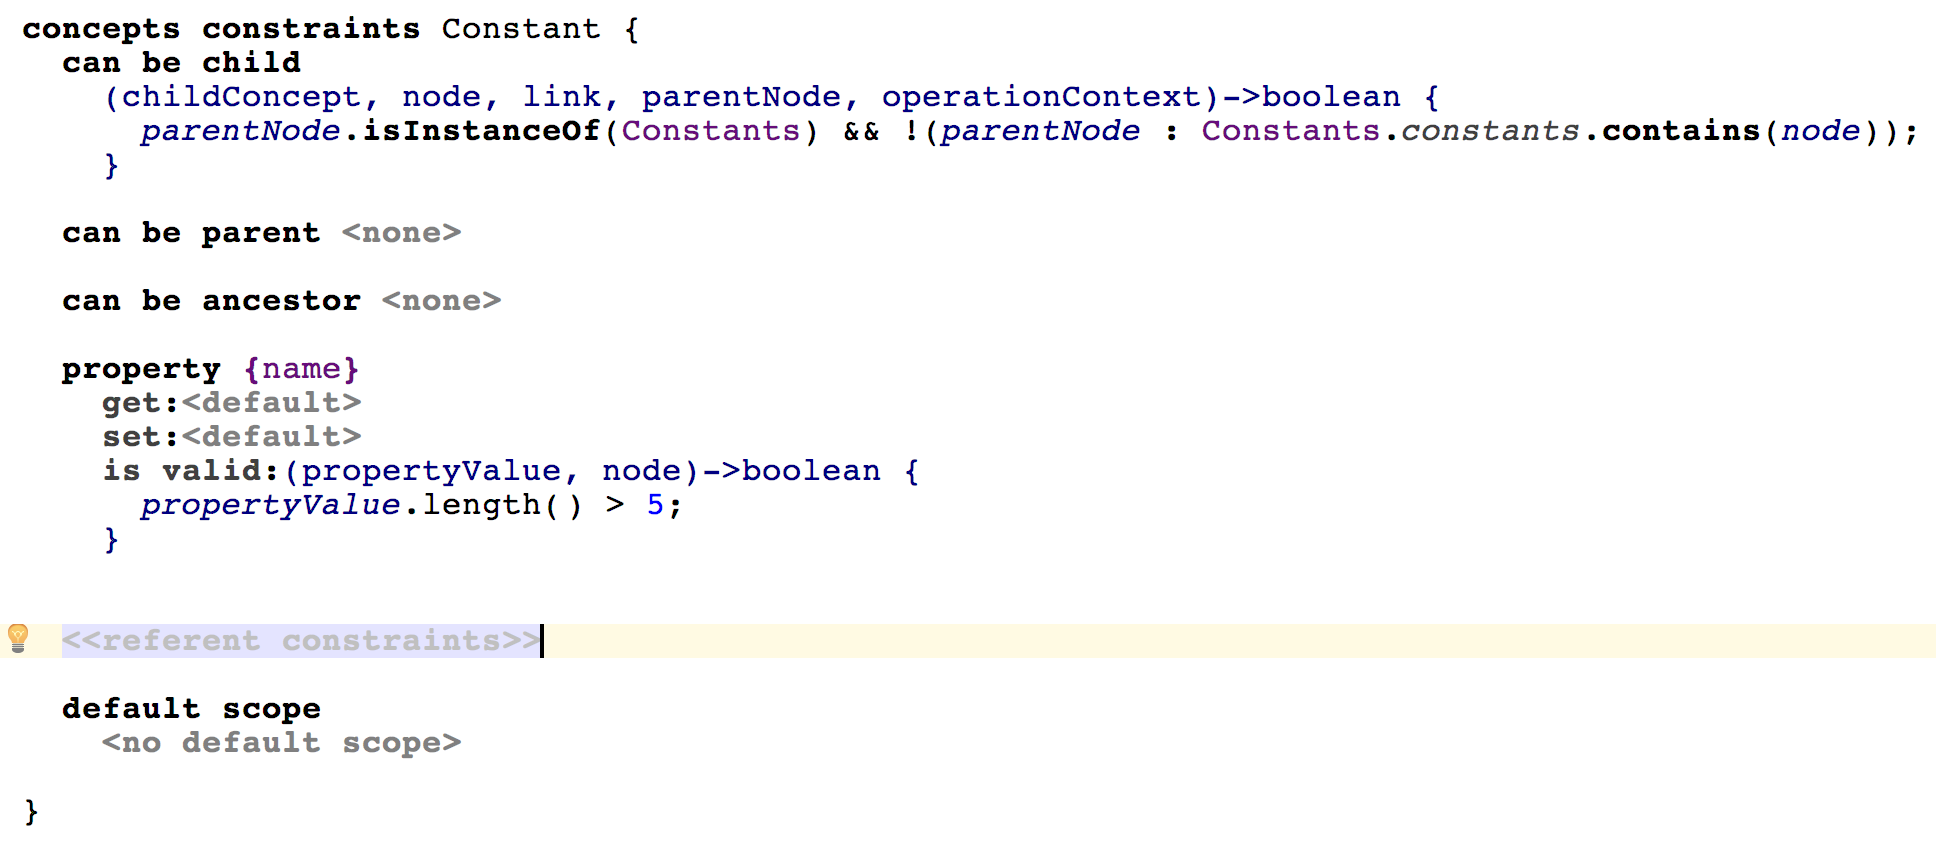
\includegraphics [scale=0.8] {Constraints}
			\caption{Пример ограничения для концепции} 
			\label{img:Constraints}  
		\end{figure}
	
		Пакет позволяет определить три типа ограничений:
		\begin{enumerate}
			\item Ограничения на типы связи с другими концепциями:
			\begin{enumerate}
				\item быть ребёнком,
				\item быть родителем,
				\item быть предком,
				\item быть корневым элементом.
			\end{enumerate}
			\item Ограничения для каждого параметра:
			\begin{enumerate}
				\item функция получения значения,
				\item функция задания значения,
				\item функция проверки корректности.
			\end{enumerate}
			\item Ограничение на ссылки:
			\begin{enumerate}
				\item функция, вызываемая при каждом изменении ссылки,
				\item множество узлов, на которые можно сослаться,
				\item функция проверки корректности
				\item настройки отображения ссылки.
			\end{enumerate}
		\end{enumerate}
	
		Все ограничения описываются в виде функций на языке \textit{Base Language}.
		
	\subsection{Редактор}
		Для того, чтобы определить удобную структуру кода, описывающего концепцию, можно воспользоваться пакетом редакторов, предоставляемым MPS.~\cite{mpssource}
		
		Редактор отображает узел и позволяет пользователю изменять, заменять, удалять его и так далее. Узлы различных концепций имеют разные редакторы. 
		
		В MPS, редактор состоит из клеток, которые сами по себе содержат другие клетки, некоторый текст или компонент пользовательского интерфейса. Каждый редактор имеет свою концепцию, для которого он определен. Концепция не может иметь более одного редактора. Если редактора нет, MPS воспользуется редактором ближайшего предка этой концепции, которая имеет редактор. 
		
		\begin{figure}[ht] 
			\center
			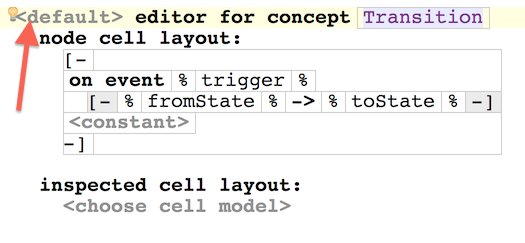
\includegraphics {editor}
			\caption{Пример описания редактора} 
			\label{img:editor}  
		\end{figure}
		
		Для описания редактора определенной концепции, MPS использует специальный язык \textit{Editor Language}. Как можно увидеть, MPS применяет принципы языково-ориентированного программирования сам к себе. 
		
		Описание редактора состоит из описаний таблицы для хранения значений полей. Например, если вы хотите, чтобы ваш редактор состоял из уникальной клетки с неизменяемым текстом, необходимо создать в вашем описании редактора постоянную клеточную модель и указать этот текст. Типы ячеек определены в документации. Пример продемонстрирован на рис. \ref{img:editor}.
		

		
\chapter{Проектирование языка}
	\section{Определение структуры языка}
		
		На основе описания ДВС составим модель концепций и их связей и представим её в виде АСД (рис. \ref{img:dcn-AST}). Здесь аналогично рис. \ref{img:AST}, связи без направления обозначают отношение родительских концепции к дочерней, где родитель находится выше дочерней концепции, а направленные связи обозначают ссылку на концепцию.
		
		\begin{figure}[ht] 
			\center
			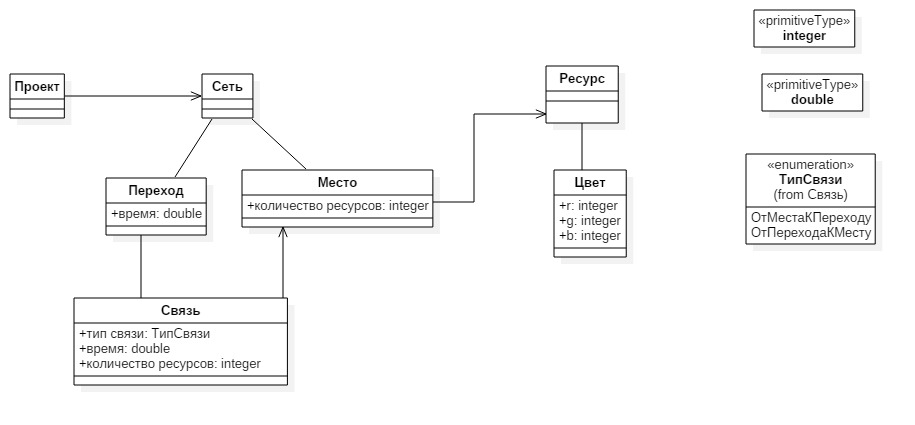
\includegraphics [scale=0.5] {dcn-AST}
			\caption{АСД языка ДВС} 
			\label{img:dcn-AST}  
		\end{figure}
	
		Как видно из схемы, можно выделить 2 интерфейса. Первый содержит параметр -- время выполнения и называется <<исполняемый>>. Второй содержит параметр -- количество ресурсов и называется <<держатель ресурсов>>.
	
		Реализацию концепций можно увидеть в прил. \ref{AppendixA}.
		
		    
	\section{Ограничения}
		Опишем ограничения для реализованных в предыдущем пункте концепций и концептуальных интерфейсов:
		\begin{enumerate}
			\item \textbf{Цвет:} все компоненты цвета должны находиться в диапазоне от 0 до 255 в соответствии с цветовой моделью RGB.
			\item \textbf{Ресурсы:} все ресурсы должны иметь уникальные имена внутри модели
			\item \textbf{Держатель ресурсов:} количество ресурсов должно быть неотрицательно.
			\item \textbf{Исполняемый:} время исполнения должно быть неотрицательно.
			\item \textbf{Место:} имя места должно быть уникально внутри содержащей его сети.
			\item \textbf{Сеть:} имя сети должно быть уникально внутри модели.
			\item \textbf{Связь:} может связывать переход только с местом, описанным в той же сети. Если тип связи <<Контролирующая>>, ресурс места должен быть \textit{Nat}.
			\item \textbf{Переход:} если не связан с сетью-объектом, не может иметь контролирующих связей.
		\end{enumerate}
			
		Реализация ограничений описана в прил. \ref{AppendixB}
		
	\section{Редактор}
		Редактор для каждой описанной концепции описан в прил. \ref{AppendixC}.
		
	\section{Тестовый проект}
		Создадим тестовый проект, содержащий 2 сети-объекта и 2 ресурса. Результат можно увидеть на рис. \ref{fig:project-tree}.	

		\begin{figure}[th]
			\centering
			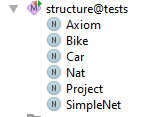
\includegraphics[width=0.3\linewidth]{images/test-project/project-tree}
			\caption{Файлы тестового проекта.}
			\label{fig:project-tree}
		\end{figure}
	
		\lstinputlisting[language={Java},caption={Проект Project},label={list:Project}]{listings/test/Project.txt}
		
		\lstinputlisting[language={Java},caption={Сеть Axiom},label={list:Axiom}]{listings/test/Axiom.txt}
		\lstinputlisting[language={Java},caption={Сеть SimpleNet},label={list:SimpleNet}]{listings/test/SimpleNet.txt}
		
		\lstinputlisting[language={Java},caption={Ресурс Car},label={list:Car}]{listings/test/Car.txt}
		\lstinputlisting[language={Java},caption={Ресурс Bike},label={list:Bike}]{listings/test/Bike.txt}
		\lstinputlisting[language={Java},caption={Ресурс Nat},label={list:Nat}]{listings/test/Nat.txt}
		
		Представление распознаётся, как корректное.
		
		\subsection{Некорректный ресурс}
			Попробуем создать ресурс с занятым именем и некорректными параметрами цвета. Как видно на рис. \ref{fig:resource-test}, имя и недопустимый параметр подсвечены красным, что говорит о том, что анализатор распознал ошибку.
		
			\begin{figure}[th]
				\centering
				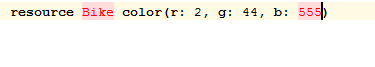
\includegraphics[width=0.7\linewidth]{images/test-project/resource}
				\caption{Ресурс с некорректными данными}
				\label{fig:resource-test}
			\end{figure}
	
		\subsection{Ограничения на связь}
			В соответствии с ограничениями, определёнными выше, связь может ссылаться только на место, определённое в той же сети. Воспользуемся для проверки ограничения функцией определения возможных значений поля в среде MPS, нажав \textit{Ctrl+Space}. Как видно из рис. \ref{fig:connection-test}, тест пройден.
			
			\begin{figure}[th]
				\centering
				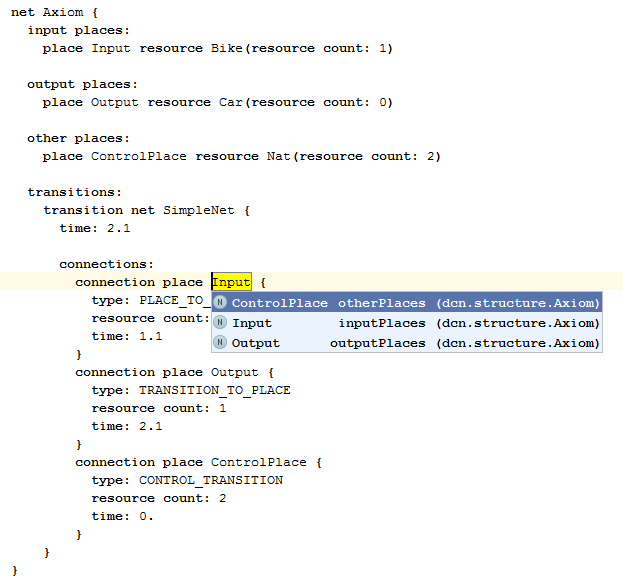
\includegraphics[width=0.7\linewidth]{images/test-project/connection}
				\caption{Возможные значения ссылки на место у связи.}
				\label{fig:connection-test}
			\end{figure}
			\FloatBarrier
			
			Также проверим корректность проверки времени. На рис. \ref{fig:time} приведены результаты.
	
			\begin{figure}[th]
				\centering
				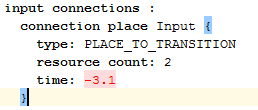
\includegraphics[width=0.4\linewidth]{images/test-project/time}
				\caption{Подсветка некорректного значения времени}
				\label{fig:time}
			\end{figure}
			\FloatBarrier
			\clearpage
		
			Убедимся, что нельзя задать контролирующую связь с местом, ресурс которого отличен от <<Nat>> (рис. \ref{fig:control-connection}).
			
			\begin{figure}[th]
				\centering
				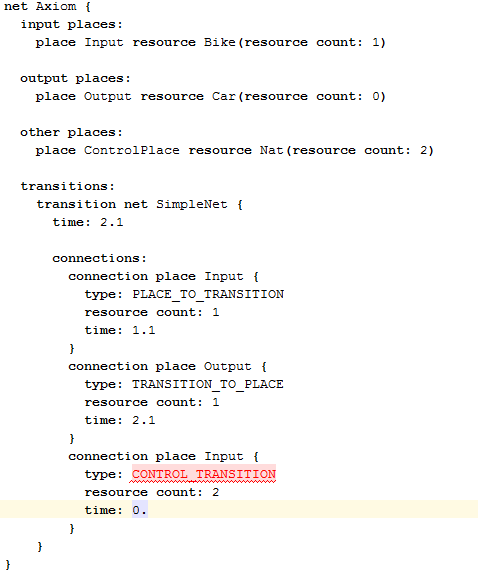
\includegraphics[width=0.7\linewidth]{images/test-project/control-connection}
				\caption{Контролирующая связь, связанная с местом, тип которого отличен от <<Nat>>}
				\label{fig:control-connection}
			\end{figure}
			\FloatBarrier
			\clearpage
		
			\subsection{Некорректная реализация перехода}
			Удостоверимся, что нельзя задать контролирующую связь для перехода, не связанного с сетью-объектом (рис. \ref{fig:control-without-net}).
			\begin{figure}[th]
				\centering
				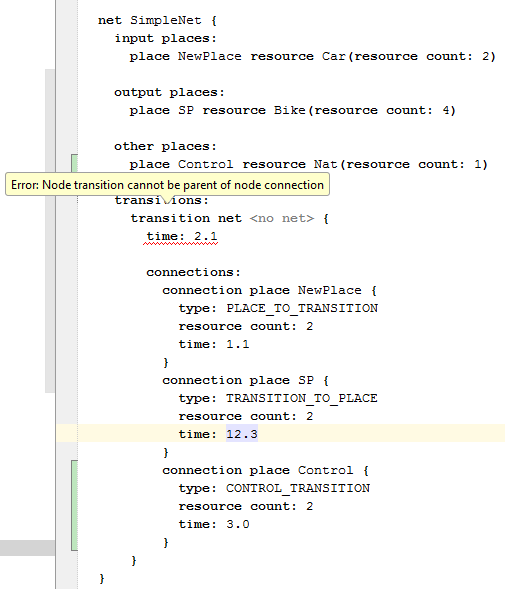
\includegraphics[width=0.7\linewidth]{images/test-project/control-without-net}
				\caption{Переход, не связанный с сетью-объектом, но имеющий контролирующий переход.}
				\label{fig:control-without-net}
			\end{figure}
		
	
	%TODO Визуализировать с помощью https://github.com/DSLFoundry/mps-langvis, если будет время  % Текст работы
	\chapter*{Заключение}						% Заголовок
\addcontentsline{toc}{chapter}{Заключение}	% Добавляем его в оглавление

%% Согласно ГОСТ Р 7.0.11-2011:
%% 5.3.3 В заключении диссертации излагают итоги выполненного исследования, рекомендации, перспективы дальнейшей разработки темы.
%% 9.2.3 В заключении автореферата диссертации излагают итоги данного исследования, рекомендации и перспективы дальнейшей разработки темы.
%% Поэтому имеет смысл сделать эту часть общей и загрузить из одного файла в автореферат и в диссертацию:

Основные результаты работы заключаются в следующем.
%% Согласно ГОСТ Р 7.0.11-2011:
%% 5.3.3 В заключении диссертации излагают итоги выполненного исследования, рекомендации, перспективы дальнейшей разработки темы.
%% 9.2.3 В заключении автореферата диссертации излагают итоги данного исследования, рекомендации и перспективы дальнейшей разработки темы.
\begin{enumerate}
	\item Изучены возможности MPI для реализации многопоточности в рамках одного узла.
	\item Спроектирована общая архитектура вычислительного узла ЯГСПП.
	\item Разработана базовая библиотека для реализации ЯГСПП в различных средах.
	\item На основе базовой библиотеки разработана библиотека для реализации ЯГСПП в среде MPI.
\end{enumerate}


Полученные знания и заключения позволят в краткий срок реализовать описанную систему, а также сделать её гибкой и расширяемой. % Заключение
	\clearpage                                  % В том числе гарантирует, что список литературы в оглавлении будет с правильным номером страницы
\phantomsection
\addcontentsline{toc}{chapter}{\bibname}	% Добавляем список литературы в оглавление
%\hypersetup{ urlcolor=black }               % Ссылки делаем чёрными
%\providecommand*{\BibDash}{}                % В стилях ugost2008 отключаем использование тире как разделителя 
\urlstyle{rm}                               % ссылки URL обычным шрифтом
\insertbibliofull                          % Подключаем Bib-базы
\urlstyle{tt}                               % возвращаем установки шрифта ссылок URL
%\hypersetup{ urlcolor={urlcolor} }          % Восстанавливаем цвет ссылок % Список литературы
%	\appendix
%% Правка оформления ссылок на приложения:
%http://tex.stackexchange.com/questions/56839/chaptername-is-used-even-for-appendix-chapters-in-toc
%http://tex.stackexchange.com/questions/59349/table-of-contents-with-chapter-and-appendix
%% требует двойной компиляции
\addtocontents{toc}{\def\protect\cftchappresnum{\appendixname{} }%
\setlength{\cftchapnumwidth}{\widthof{\cftchapfont\appendixname~Ш\cftchapaftersnum}}%
}
%% Оформление заголовков приложений ближе к ГОСТ:
\sectionformat{\chapter}[display]{% Параметры заголовков разделов в тексте
    label=\chaptertitlename\ \thechapter,% (ГОСТ Р 2.105, 4.3.6)
    labelsep=20pt,
}
\renewcommand\thechapter{\Asbuk{chapter}} % Чтобы приложения русскими буквами нумеровались
   % Предварительные настройки для правильного подключения Приложений
\chapter{Примеры вставки листингов программного кода} \label{AppendixA} % Приложения
\end{document}
